
\section{Enhancer Linking by Methylation/Expression Relationships (ELMER)}

Motivated by the discovery of transcriptional enhancers in tissue DNA methylation data \cite{berman2012ng}, and subsequent approaches to linking these enhancers to transcriptional targets using a chromQTL approach \cite{aran2013dna} (reviewed in \citeauthoronline{yao2015inferring}), \citeauthoronline{yao2015inferring} developed the the R/Bioconductor  \textit{ELMER} (Enhancer Linking by Methylation/Expression Relationships) package, a tool which infers regulatory element landscapes and transcription factor networks from cancer methylomes.

This tool combined DNA methylation and gene expression data from human tissues to infer multi-level cis-regulatory networks through several steps which included the identification of distal enhancer probes with significantly altered DNA methylation levels in primary tumor tissues compared to normal tissues, followed by the identification of putative target genes, and a comprehensive gene regulatory network analysis which combined transcription factor motifs at the altered enhancers with TF expression to identify the underlying master regulators. This approach identified several known and unknown master regulators in TCGA data, such as \sigla{GATA3}{GATA-binding protein 3} and \sigla{FOXA1}{Forkhead box protein A1} in breast cancer, and \sigla{P63}{tumor protein p63} and \sigla{SOX2}{Sex determining region Y-box 2} in squamous cell lung carcinoma \cite{yao2015inferring,silva2016tcga}.

Based on user feedback and a full review of the source code, we identified and implemented a number of software improvements, which are summarized in table \ref{tab:summary}: (i) The original package contained no standard data structure to handle multiple assays (DNA methylation, gene expression, and clinical data), which would be required for an integrative genomic data analysis. Recently, the Bioconductor team provided such a data structure through the \href{http://bioconductor.org/packages/MultiAssayExperiment/}{MultiAssayExperiment} package. (ii) All auxiliary databases (human TF list, classification of TF in families, gene annotation, DNA methylation annotation and motif occurrences within probe sites) used in the package were created and maintained manually, thereby making the upgrade process laborious; thus, we automated this process. (iii) The package was developed to analyze primary tumor tissue samples compared to normal tissues samples, thus not allowing arbitrary subgroups to be compared (for instance mutants vs. non-mutants, treated vs. untreated, etc.) (iv) Our original approach used known epigenomic markers for enhancers to constrain the genomic regions searched for differential methylation. However, this selection could limit our algorithm to identifying regulatory networks for tissue types that exist in the epigenomic databases; we found this constraint problematic, and thus now search \textit{all} distal regulatory regions without any such filter. (v) The function used to download data from The Cancer Genome Atlas (TCGA) data portal \cite{tomczak2015cancer} broke when the TCGA site was shutdown and its data transferred to The NCI's Genomic Data Commons (GDC) \cite{grossman2016toward}; we now have a more general data provider interface that supports GDC as the default provider. (vi) The package only supported data aligned to Genome Reference Consortium GRCh37 (hg19), and we now provide support for Genome Reference Consortium GRCh38 (hg38). (vii) There was no support to the recent HumanMethylationEPIC (EPIC) array. In addition to the specific improvements listed above, we substantially re-wrote most of the code to be more efficient and maintainable,  also most of the output plots generated were improved.

\bgroup
\def\arraystretch{2.0}%  1 is the default, change whatever you need

\begin{table}[h!]
\footnotesize
\centering
\caption{Main differences between ELMER old version (v.1) and the new version (v.2)}
\label{tab:summary}
\begin{tabular}{|p{4cm}|p{5cm}|p{6cm}|}
\toprule
\toprule
\multicolumn{1}{|c|}{\textbf{Features}} & \multicolumn{1}{|c|}{\textbf{ELMER Version 1}} & \multicolumn{1}{|c|}{\textbf{ELMER Version 2}}   \\ \midrule \midrule
Primary data structure   & mee object (custom data structure)   & MAE object (Bioconductor data structure) \\ \hline
Auxiliary data  & Manually created  & Programmatically created \\  \hline
Number of human TFs & 1,982  & 1,987 (Uniprot database)  \\  \hline
Number of TF motifs  & 91  & 771  (HOCOMOCO v11 database)  \\  \hline
TF classification    & 78 families & 82 families and 331 subfamilies \newline(TFClass database) \\  \hline
Analysis performed  & Normal vs tumor samples & Group 1 vs group 2  \\  \hline
Statistical grouping   & unsupervised only & unsupervised or supervised using labeled groups   \\  \hline
TCGA data source   & The Cancer Genome Atlas (TCGA) (not available)          & The NCI's Genomic Data Commons (GDC) \\  \hline
Genome of reference   & GRCh37 (hg19)   & GRCh37 (hg19)/GRCh38 (hg38)          \\ \hline
DNA methylation platforms  & HumanMethylation450   & HumanMethylationEPIC and HumanMethylation450   \\  \hline
Graphical User interface (GUI) & None & TCGAbiolinksGUI \\
\bottomrule
\end{tabular}
\end{table}
\egroup

In this section, we present a new version of the R \textit{ELMER} package,
which addresses all the issues described above. We start out by the detailed explanation
of the algorithms, follow by a case of study using breast Cancer data used as an
illustration of the use of the tool.


%The new version of \textit{ELMER} (v2.0.0) is available as an R/Bioconductor package at \burl{https://github.com/tiagochst/ELMER}. And, the new version of \textit{ELMER.data} (v2.0.0), which provides auxiliary data required to perform the analysis, is available at
%\burl{https://github.com/tiagochst/ELMER.data}.

\subsection{Implementation}

Here we describe each of following analysis steps shown in figure \ref{fig:elmerworkflow}.

\begin{itemize}
    \item Organize data as a \textit{MultiAssayExperiment} object
	\item Identify distal probes with significantly different DNA methylation
   level when comparing two sample groups.
	\item Identify putative target genes for differentially methylated
   distal probes, using methylation vs. expression correlation
	\item Identify enriched motifs for each probe belonging
  to a significant probe-gene pair
	\item Identify master regulatory Transcription Factors (TF)
   whose expression associate with DNA methylation changes at multiple regulatory regions.
\end{itemize}


%\begin{landscape}
\tikzstyle{container} = [
    rectangle,
    draw,
    inner sep=0.2 cm,
    dashed
]
\tikzstyle{start} = [circle,
					 minimum size=2mm,
                     rounded corners=3mm,
					 very thick,
                     draw=green!50!black,
                     top color=green!50!black,
                     bottom color=green!50!black, 
                     text=white,
                     font=\tiny]

\tikzstyle{end} = [circle,
				  minimum size=2mm,
                  rounded corners=3mm,
                  very thick,draw=red!50!black, 
                  top color=red!50!black,
                  bottom color=red!50!black, 
                  text=white,
                  font=\tiny]

\tikzstyle{function} = [rectangle,
						minimum size=6mm,
                        rounded corners=3mm,
                        very thick,
                        draw=black!50, 
                        top color=white,
                        bottom color=white,
                        font=\itshape\footnotesize]

\tikzstyle{datain} = [
	rectangle, 
	rounded corners, 
    minimum width=3cm, 
    minimum height=0.5cm,
    text centered,
    font=\footnotesize, 
    draw=green!50!black, 
    fill=white, 
    text=black
]
                      
\tikzstyle{dataaux} = [
	rectangle, 
    rounded corners, 
    minimum width=3cm, 
    minimum height=0.5cm,
    text centered,
    font=\footnotesize,
    draw=orange, 
    fill=white, 
    text=black
]
                       
\tikzstyle{dataout} = [
	rectangle, 
	rounded corners, 
    minimum width=3cm, 
    minimum height=0.5cm,
    text centered,
    font=\footnotesize, 
    draw=blue, 
    fill=white, 
    text=black
]

% Pacakge labels
\tikzstyle{arrow} = [
	thick,
    ->,
    >=stealth,
    -latex',
    draw,
    rounded corners
]

\tikzstyle{labelelmer}=[
	rectangle,
    draw,
    fill=black!50!red,
    draw = black,
    minimum width=450pt,
    minimum height=1.5em,
    text=white,
    rotate = 90, 
    label={[rotate=90]center:\textcolor{white}{\textbf{ELMER package}}}
]

\tikzstyle{labeltcgabiolinks}=[
	rectangle,
	draw,
    fill=black!50!blue,
    draw = black,
    minimum width=420pt,
    minimum height=1.5em,
    text = green,
    rotate = 90, 
    label={[rotate=270]center:\textcolor{white}{\textbf{TCGAbiolinks/TCGAbiolinksGUI packages}}}
]


\tikzstyle{labelfuncivar}=[
	rectangle,
	draw,
    fill=black!20!orange,
    draw = black,
    xshift = -0.0cm,
    minimum width=480pt,
    minimum height=1.5em,
    text=white,
    rotate = 0, 
    label={[rotate=0]center:\textcolor{white}{\textbf{StateHub/StatePaintR/funcivar package}}}
]
\tikzstyle{labelgdc}=[
	rectangle,
	draw,
    fill=black!50!gray,
    draw = black,
    minimum width=167pt,
    minimum height=1.5em,
    text=white,
    yshift = 0.10cm,
    xshift = 0.1cm,
    rotate = 0, 
    label={[rotate=0]center:\textcolor{white}{\textbf{GDC database}}}
]
\tikzstyle{every annotation}=[fill=white, font=\sf \small, scale=0.5, text width=4cm, inner sep=2mm, text=black,draw = orange]


\begin{figure}[!ht]
\centering
  \resizebox{0.95\textwidth}{!}{%
\begin{tikzpicture}[node distance = 1.5cm, auto, shorten >=1pt,thick,font=\itshape\footnotesize]
\linespread{0.8}{
%\node (start) [start] {START};
\node (func1) [function, yshift = -0.5cm] {\textit{createMAE}};
\node [datain, right of=func1, yshift = 0.5cm, xshift = 2cm] (dna) {DNA methylation object};
\node [datain, right of=func1, yshift = -0.5cm, xshift = 2cm] (exp) {Gene expression object};
\node (out1) [dataout, below of=func1, yshift = -0.3cm,text width=3cm] {Multi Assay Experiment object};
\node (func2) [function, below of = out1] {get.diff.meth};
%\node (out2) [dataout, below of=func2, yshift = 0.3cm] {List of differently methylated probes};
\node (func3) [function, below of=func2] {GetNearGenes};
%\node (out3) [dataout, below of=func2, yshift = 0.3cm] {List of near genes for differently methylated probes};
\node (func4) [function, below of=func3] {get.pair};
%\node (out4) [dataout, below of=func4, yshift = 0.3cm] {List of pairs: differently expressed gene and differently methylated probes};
\node (func5) [function, below of=func4, yshift = -0.5cm] {get.enriched.motif};
%\node (out5) [dataout, below of=func5, yshift = 0.3cm] {List of enriched motifs};
\node (func6) [function, below of=func5] {get.TFs};
\node (func7) [function, below of=func6,yshift = -0.5cm] {TF.survival};
%\node (out5) [dataout, below of=func5, yshift = 0.3cm] {List of regulator};
\node [dataaux, left of=func5, xshift =-3cm] (elmerdata1) {Probes.motif};
%\node [dataaux, above of=elmerdata1] (enhancer) {enhancer};
\node [dataaux, left of=func6, yshift = 0.0cm, xshift =-3cm] (elmerdata2) {motif.relevant.TFs};
\node [dataaux, left of=func6, yshift = -1.0cm, xshift =-3cm] (elmerdata3) {human.TFs};
%\node (end) [end, below of=func7] {END};
\node (func8) [function, left of=func1,yshift = -3cm,xshift = -3cm] {get.feature.probe};
\node (probes) [datain, left of=func1,xshift = -3cm] {distal probes};
\node [dataaux, below of=func8] (tss) {ENSEMBL TSS};
\node [dataaux, below of=tss] (probesmetadata) {Probes metadata};


% funcvat
\node (funciVar) [function, below of=func7, xshift = 3cm, yshift = -1.4cm] {enrich.segments};
\node [dataaux, left of=funciVar,xshift = -2cm] (statehub) {Statehub tracks};
%\node [dataaux, left of=statehub,xshift = -2cm, yshift = 0.2cm] (encode) {ENCODE};
%\node [dataaux, left of=statehub,xshift = -2cm, yshift = -0.4cm] (roadmap) {ROADMAP};
%\node [dataaux, left of=statehub,xshift = -2cm, yshift = 0.8cm] (blueprint) {BLUEPRINT};
%\draw [arrow,dashed,draw=orange] (encode.east) -- (statehub.west);
%\draw [arrow,dashed,draw=orange] (roadmap.east) -- (statehub.west);
%\draw [arrow,dashed,draw=orange] (blueprint.east) -- (statehub.west);

\draw [arrow,dashed,draw=orange] (statehub.east) -- (funciVar.west);

\draw [arrow] (func4) -- ++(4.9,0) -- ++(0,-1) |- node {} (funciVar);

% Draw edges
%\path [arrow] (start) -- (func1);
\path [arrow,dashed,draw=green!50!black] (dna) |- (func1);
\path [arrow,dashed,draw=green!50!black] (exp) |- (func1);
\draw [arrow,dashed,draw=blue] (out1.west) -- ++(-.5,0) -- ++(0,-1) |- (func4.west);
\draw [arrow,dashed,draw=blue] (out1.west) -- ++(-.5,0) -- ++(0,-1) |- (func6.west);
\draw [arrow] (func1) -- (out1);
\draw [arrow] (out1) -- (func2);
\draw [arrow] (func2) -- node {} (func3);
\draw [arrow] (func3) -- (func4);
\draw [arrow] (func4) -- node {} (func5);
\draw [arrow] (func5) -- node {}(func6);
\draw [arrow] (func6) -- (func7);
%\draw [arrow] (func7) -- (end);
\draw [arrow,dashed,draw=orange] (elmerdata1) -- node {} (func5);
\draw [arrow,dashed,draw=orange] (elmerdata2.east) -- (func6.west);
\draw [arrow,dashed,draw=orange] (elmerdata3.east) -- ++(.5,0) -- ++(0,0.2) |- (func6.west);
%\draw [arrow,dashed,draw=orange] (enhancer.north) -- (func8.south);
\draw [arrow,dashed,draw=orange] (tss.north) -- (func8.south);
\draw [arrow,dashed,draw=orange] (probesmetadata.east) -- ++(.1,0) -- ++(0,0.2) |- (func8.east);
\path [arrow,dashed,draw=green!50!black] (probes) -- (func1);
\draw [arrow] (func8.north)  --  (probes);

% Containers
\node [container, 
       fit=(exp)(dna)(func1)(probes), 
       label={[font=\scriptsize,anchor=east] west:Data input}]
       (container1){};
\node [container, 
	   fit=(func2), 
       label={[font=\scriptsize,anchor=west,name=lfunc1] east:{\parbox[c]{4.0cm}{Identifying differentially\\ methylated probes}}}]
       (container2){};
\node [container, 
       fit=(func3)(func4), 
	   label={[font=\scriptsize,anchor=west,name=lfunc2] east:{\parbox[c]{4.0cm}{Identifying putative \\probe-gene pairs}}}]
       (container3){};
\node [container, 
 	   fit=(func5), 
       label={[font=\scriptsize,anchor=west] east:{\parbox[c]{4.0cm}{Motif enrichment\\ analysis}}}]
       (container4){};
\node [container, 
       fit=(func6), 
       label={[font=\scriptsize,anchor=west] south east:Identifying regulatory TFs}]
       (container5){};
\node [container, 
       fit=(elmerdata1)(elmerdata1), 
       label={[name=l1,font=\scriptsize,anchor=east] west:ELMER.data}]
       (container6){};
%\node[draw,text width=3cm, above of = elmerdata1]{ELMER.data};
\node [container, 
	   fit=(func8)(probesmetadata), 
	   label={[name=l3,font=\scriptsize,anchor=east] west:{\parbox[r]{2.0cm}{Select probes \\$\pm 2Kb$  distant \\ from TSS}}}]
       (container8){};

\node [container, 
       fit=(elmerdata2), 
       label={[name=l2,font=\scriptsize,anchor=east] west:TFClass database}]
       (container7){};
\node [container, 
	   fit=(elmerdata3), 
	   label={[name=l3,font=\scriptsize,anchor=east] west:Uniprot database}]
       (container8){};
\node [draw,  
       minimum height=450pt,
	   minimum width=450pt,
       fit=(l1)(exp)(dna)(elmerdata3)(l2)(lfunc1)(lfunc2)]
       (container9){};
\node at (container9.west) [labelelmer] {};
  
%------------------------------ TCGAbiolinks
\node (GDCprepare) [function, right of = func1, yshift =-1.3cm,xshift =8.8cm] {\textit{GDCprepare}};
\node (GDCdownload) [function, above of = GDCprepare,yshift =-0.4cm] {\textit{GDCdownload}};
\node (GDCquery) [function, above of = GDCdownload,yshift =-0.4cm] {\textit{GDCquery}};
\node (TCGAanalysesurvival) [function, right of = func7,xshift =7.8cm] {\textit{TCGAanalyse\_survival}};
\node (TCGAanalyzeEAcomplete) [function, right of = func4,yshift =0.4cm,xshift =7.8cm] {\textit{TCGAanalyze\_EAcomplete}};
\node (TCGAanalyzePathview) [function, right of = func4,yshift =-0.7cm,xshift =7.8cm] {\textit{TCGAanalyze\_Pathview}};
\node (TCGAvisualizeoncoprint) [function, right of = func4,yshift =-1.8cm,xshift =7.8cm] {\textit{TCGAvisualize\_oncoprint}};

\draw [arrow] (GDCquery) -- node {}(GDCdownload);
\draw [arrow] (GDCdownload) -- (GDCprepare);
\draw [arrow] (GDCprepare.west) -- ++(-0.3,0) -- ++(0,0.2) |- (dna.east);
\draw [arrow] (GDCprepare.west) -- ++(-0.3,0) -- ++(0,0.2) |- (exp.east);

\node (subtypeinfo) [dataaux, below of = GDCprepare,yshift =0.6cm] {Subtype information};
\node (molecularinfo) [dataaux, below of = subtypeinfo,yshift =0.6cm] {Molecular data};
\node (clinicalinfo) [dataaux,  below of = molecularinfo,yshift =0.6cm] {Clinical data};
\node (mafinfo) [dataaux, below of = clinicalinfo,yshift =0.6cm] {Mutation data};

\draw [arrow,dashed,draw=orange] (mafinfo.east) -- ++(0.5,0) -- ++(0,-0.2) |-    (TCGAvisualizeoncoprint.east);
\draw [arrow,dashed,draw=orange] (clinicalinfo.east)  -- ++(0.3,0) -- ++(0,0.2) |-   (GDCprepare.east);
\draw [arrow,dashed,draw=orange] (subtypeinfo.east)   -- ++(0.2,0) -- ++(0,0.2) |-   (GDCprepare.east);
\draw [arrow,dashed,draw=orange] (molecularinfo.east) -- ++(0.3,0) -- ++(0,0.2) |-  (GDCprepare.east);
\node [draw,  
       minimum height=420pt,
       minimum width=170pt, 
       xshift = 0.25cm,
       yshift = -0.25cm,
       fit=(TCGAanalyzeEAcomplete)(GDCquery)(TCGAanalysesurvival)(clinicalinfo)(subtypeinfo)](container10){};
\node at (container10.east) [labeltcgabiolinks] {};
\draw [latex'-latex',double] (TCGAanalysesurvival) --  (func7);
\draw [arrow] (func4.east)  -- ++(4.4,0) -- ++(0,0.2) |-  (TCGAanalyzeEAcomplete);
\draw [arrow] (func4.east)  -- ++(4.4,0) -- ++(0,-0.2) |-  (TCGAanalyzePathview);
\draw [arrow] (func4.east)  -- ++(4.4,0) -- ++(0,-0.2) |-  (TCGAvisualizeoncoprint);
\draw [arrow] (func6.east)  -|   (TCGAvisualizeoncoprint.south);
%------------------------------ 
\node [labelgdc, above of = GDCquery,xshift=-0.30cm,yshift=-0.05cm] (gdc) {};
\draw [latex'-latex',double] (GDCquery) --  (gdc.300);

\draw [draw,dashed] (gdc.188) |- (GDCdownload.west);
\draw [arrow,dashed] (gdc.188) |- (mafinfo.west);
\draw [arrow,dashed] (gdc.188) |- (clinicalinfo.west) ;
\draw [arrow,dashed] (gdc.188) |- (molecularinfo.west) ;
}

\tikzstyle{labelencode}=[
	rectangle,
	draw,
    fill=black!50!gray,
    draw = black,
    minimum width=150pt,
    minimum height=1.5em,
    text=white,
    yshift = 0.10cm,
    xshift = 0.1cm,
    rotate = 0, 
    label={[rotate=0]center:\textcolor{white}{\textbf{ENCODE database}}}
]
\tikzstyle{labelroadmap}=[
	rectangle,
	draw,
    fill=black!50!gray,
    draw = black,
    minimum width=150pt,
    minimum height=1.5em,
    text=white,
    yshift = 0.10cm,
    xshift = 0.1cm,
    rotate = 0, 
    label={[rotate=0]center:\textcolor{white}{\textbf{ROADMAP database}}}
]
\tikzstyle{labelblueprint}=[
	rectangle,
	draw,
    fill=black!50!gray,
    draw = black,
    minimum width=150pt,
    minimum height=1.5em,
    text=white,
    yshift = 0.10cm,
    xshift = 0.1cm,
    rotate = 0, 
    label={[rotate=0]center:\textcolor{white}{\textbf{BLUEPRINT database}}}
]

\node [draw,  
       minimum height=6.52em,
       minimum width=480pt, 
       xshift = 1.60cm,
       yshift = 0.05cm,
       fit=(funciVar)(funciVar)](containerFunciVar){};
\node at (containerFunciVar.south) [labelfuncivar] {};


\node [labelencode, right of = statehub,xshift=-8.20cm,yshift=-0.15cm] (encode) {};
\node [labelroadmap, below of = encode,xshift=-0.1cm,yshift=0.7cm] (roadmap) {};
\node [labelblueprint, above of = encode,yshift=-0.8cm,xshift=-0.1cm] (blueprint) {};
%\draw [latex'-latex',double] (encode.180) --  (containerFunciVar.0);
\draw [double,->] (encode.0) --  (statehub.180);
\draw [double,->] (roadmap.0) -- ++(1.4,0) |-   (statehub.180);
\draw [double,->] (blueprint.0) -- ++(1.4,0) |-  (statehub.180);
\end{tikzpicture}
  }%
  
  \caption[ELMER workflow]{ELMER workflow: ELMER receives as input a DNA methylation object, a gene expression object (a matrix or a SummarizedExperiment object) and a Genomic Ranges (GRanges) object with distal probes to be used as filter which can be retrieved using the \textit{get.feature.probe} function. The function \textit{createMAE}  will create a Multi Assay Experiment object keeping only samples that have both DNA methylation and gene expression data. Genes will be mapped to genomic position and annotated using ENSEMBL database \cite{doi:10.1093/database/baw093}, while for probes it will add annotation from \citeauthor{doi:10.1093/nar/gkw967} (\href{http://zwdzwd.github.io/InfiniumAnnotation}{http://zwdzwd.github.io/InfiniumAnnotation}) . This MAE object will be used as input to the next analysis functions. First, it identifies differentially methylated probes followed by the identification of their nearest genes (10 upstream and 10 downstream) through the  \textit{get.diff.meth} and  \textit{GetNearGenes} functions respectively. For each probe, it will verify if any of the nearby genes were affected by its change in the DNA methylation level and a list of  gene and probes pairs will be outputted from \textit{get.pair} function. For the probes in those pairs, it will search for enriched regulatory Transcription Factors motifs with the  \textit{get.enriched.motif} function. Finally, the  enriched motifs will be correlated with the level of the transcription factor through the \textit{get.TFs} function. In the figure green Boxes represents user input data, blue boxes represents output object, orange boxes represent auxiliary pre-computed data and gray boxes are functions.}
  \label{fig:elmerworkflow}
\end{figure}
%\end{landscape}

\subsubsection{Organization of data as a \textit{MultiAssayExperiment} object}

To facilitate the analysis of experiments and studies with multiple samples
the Bioconductor team created the \href{http://bioconductor.org/packages/SummarizedExperiment/}{\textit{SummarizedExperiment}} class \cite{huber2015orchestrating}, a data structure able to store data and metadata for a single experiment but not for data spanning several experiments for the same sample. To overcome this problem, recently, the MultiAssay SIG (Special Interest Group) created the \href{http://bioconductor.org/packages/MultiAssayExperiment/}{MultiAssayExperiment class} \cite{mae2017} a data structure to manage and preprocess multiple assays for
integrated genomic analysis. This data structure is now an input for all main functions
of \href{https://github.com/tiagochst/ELMER}{\textit{ELMER}} and can be generated
by the \textit{createMAE} function.


To perform \textit{ELMER} analyses, users need to populate a \textit{MultiAssayExperiment}
with a DNA methylation matrix or \textit{SummarizedExperiment} object from
\sigla{HM450}{HumanMethylation450 BeadChip} or \sigla{EPIC}{MethylationEPIC BeadChip} platform;
 a gene expression matrix or SummarizedExperiment object for the same samples;
 a matrix mapping DNA methylation samples to gene expression samples; and a matrix with sample metadata (i.e. clinical data, molecular subtype, etc.). If TCGA data are used, the last two matrices will be automatically generated.
If using non-TCGA data, the matrix with sample metadata should be provided with at least a column with a patient identifier and another one identifying its group which will be used for analysis, if samples in the methylation and expression matrices are not ordered and with same names, a matrix mapping for each patient identifier their DNA methylation samples and their gene expression samples should be provided to the \textit{createMAE} function.
Based on the genome of reference selected, metadata for the DNA methylation probes, such as genomic coordinates, will be added from   \href{http://zwdzwd.github.io/InfiniumAnnotation}{\citeonline{zhou2016comprehensive}};
and metadata for gene expression and annotation is added from ENSEMBL database \cite{yates2015ensembl} using \href{http://bioconductor.org/packages/biomaRt/}{biomaRt}
\cite{durinck2009mapping}.

\subsubsection{Selecting distal probes}
Probes from HumanMethylationEPIC (EPIC) array and Infinium HumanMethylation450 (HM450)
array are removed from the analysis if they have either internal SNPs close to the $3'$
end of the probe; non-unique mapping to the bisulfite-converted genome;
or off-target hybridization due to partial overlap with non-unique elements \cite{doi:10.1093/nar/gkw967}.
This probe metadata information is
included in \href{https://github.com/tiagochst/ELMER.data}{\textit{ELMER.data}} package,
populated from the source file at \url{http://zwdzwd.github.io/InfiniumAnnotation}
\cite{doi:10.1093/nar/gkw967}.
To limit ELMER to the analysis of distal elements, probes located in regions of $\pm2 kb$
around \sigla{TSSs}{transcription start sites} were removed.

\subsubsection{Identification of differentially methylated CpGs (DMCs)}

For each distal probe, samples of each group (group 1 and group 2) are ranked by
their DNA methylation beta values, those samples in the lower quintile (20\% samples
with the lowest methylation levels) of each group are used to identify if the probe is
hypomethylated in group 1 compared to group 2, using an unpaired one-tailed t-test.
The 20\% is a parameter to the \textit{diff.meth} function called \textit{minSubgroupFrac}. For the (ungrouped) cancer case, this is set to 20\% as in \citeonline{yao2015inferring}, because we typically wanted to be able to detect a specific molecular subtype among the tumor samples; these subtypes often make up only a
minority of samples, and 20\% was chosen as a lower bound for the purposes of
statistical power (high enough sample numbers to yield t-test p-values that could
overcome multiple hypothesis corrections, yet low enough to be able to capture
changes in individual molecular subtypes occurring in 20\% or more of the cases.)
This number can be set arbitrarily as an input to the \textit{diff.meth} function
and should be tuned based on sample sizes in individual studies. In the \textit{Supervised} mode,
where the comparison groups are implicit in the sample set and labeled,
the \textit{minSubgroupFrac} parameter is set to 100\%.
An example would be a cell culture experiment with 5 replicates of the untreated cell line,
and another 5 replicates that include an experimental treatment.

To identify hypomethylated \sigla{DMCs}{differentially methylated CpGs},
a one-tailed t-test is used to rule out the null hypothesis:
$\mu_{group1} \geq \mu_{group2}$, where $\mu_{group1}$ is the
mean methylation within the lowest group 1 quintile (or another percentile
as specified by the \textit{minSubgroupFrac} parameter) and $\mu_{group2}$
is the mean within the lowest group 2 quintile. Raw p-values are adjusted
for multiple hypothesis testing using the Benjamini-Hochberg method
\cite{benjamini1995controlling}, and probes are selected when they had
adjusted p-value less than $0.01$ (which can be configured using
the \textit{pvalue} parameter). For additional stringency, probes are only
selected if the methylation difference: $\Delta = \mu_{group1} - \mu_{group2}$
was greater than $0.3$. The same method is used to identify hypermethylated DMCs,
except we use the \textit{upper} quintile, and the opposite tail in the t-test is chosen.

\subsubsection*{Identification of putative target gene(s)}

For each differentially methylated distal probe (DMC), the closest 10 upstream
genes and the closest 10 downstream genes are tested for inverse correlation between
methylation of the probe and expression of the gene (the number 10 can be changed using the \textit{numFlankingGenes} parameter). To select these genes,
the probe-gene distance is defined as the distance from the probe to the transcription
start site specified by the ENSEMBL gene level annotations \cite{yates2015ensembl} accessed via
the R/Bioconductor package \href{http://bioconductor.org/packages/biomaRt/}{biomaRt} \cite{durinck2009mapping,durinck2005biomart}. By choosing a constant number of genes to test for each probe, our goal is to avoid systematic false positives for probes in gene rich regions. This is especially important given the highly non-uniform gene density of mammalian genomes.
Thus, exactly 20 statistical tests were performed for each probe, as follows.

For each probe-gene pair, the samples (all samples from both groups) are divided into two
groups: the $M$ group, which consisted of the upper methylation quintile (the 20\%
of samples with the highest methylation at the enhancer probe), and the $U$ group,
which consists of the lowest methylation quintile (the 20\% of samples with the
lowest methylation.) The 20\% ile cutoff is a
configurable parameter \textit{minSubgroupFrac} in the \textit{get.pair} function.
As with its usage in the \textit{diff.meth} function, the default value of 20\% is
a balance, allowing for the identification of changes in a
molecular subtype making up a minority (i.e. 20\%) of cases, while also yielding
enough statistical power to make strong predictions. For larger sample sizes or
other experimental designs, this could be set even lower.

For each candidate probe-gene pair,
the Mann-Whitney U test is used to test the null hypothesis that overall gene
expression in group M is greater than or equal than that in group U.
This non-parametric test was used in order to minimize the effects
of expression outliers, which can  occur across a very wide dynamic range.
For each probe-gene pair tested, the raw p-value $P_r$ is corrected for multiple
hypothesis using a permutation approach as follows.
The gene in the pair is held constant, and \textit{x} random methylation probes are
chosen to perform the same one-tailed U test, generating a set of \textit{x} permutation
p-values $P_p$. We chose the x random probes only from among those that were
"distal" (farther than $2kb$ from an annotated transcription start site), in order
to draw these null-model probes from the same set as the probe being tested \cite{sham2014statistical}.
An empirical p-value $P_e$ value was calculated using the following formula
(which introduces a pseudo-count of 1):

\begin{equation}
	P_e = \frac{num(P_p \leq P_r)+ 1}{x+1}
\end{equation}

Notice that in the \textit{Supervised} mode, no additional filtering is
necessary to ensure that the M and U group segregate by sample group labels.
The two sample groups are segregated by definition, since these probes were
selected for their differential methylation, with the same directionality,
between the two groups.



\subsubsection{Characterization of chromatin state context of enriched probes using FunciVar}

Unlike version 1 of \textit{ELMER}, we now consider \textit{all} distal probes
in the identification of regulatory elements. DNA methylation is known to affect
several different classes of distal chromatin state element, including active
enhancers, poised enhancers, and insulators. In order to provide a functional
interpretation of the regulatory elements identified by \textit{ELMER},
we perform a chromatin state enrichment analysis of the probes within significant
probe-gene pairs, using the \textit{statePaintR} tools from the \burl{www.statehub.org} \cite{statepaintr},
along with our new FunciVar package \cite{funcivar}. Enrichment of the putative pairs
 within chromatin states is calculated against a background model that uses the distal
 probe set that the putative pairs are drawn from.

\subsubsection*{Motif enrichment analysis}
In order to identify enriched motifs and potential upstream regulatory TFs,
all probes with occurring in significant probe-gene pairs are combined for
motif enrichment analysis. \sigla{HOMER}{Hypergeometric Optimization of Motif EnRichment}
 \cite{heinz2010simple} is used to find motif occurrences in a $\pm 250bp$ region
 around each probe, using HOCOMOCO (HOmo sapiens COmprehensive MOdel COllection)
 v11 \cite{kulakovskiy2016hocomoco}. Transcription factor (TF) binding models are
 available at \burl{http://hocomoco.autosome.ru/downloads} (using the HOMER specific
 format with threshold score levels corresponding to p-value $ \leq 1^{-4}$).

For each probe set tested (i.e. the set of all probes occurring in significant probe-gene pairs),
a motif enrichment Odds Ratio and a 95\% confidence interval are calculated using following formulas:
\begin{subequations}
\begin{align}
p = \frac{a}{a + b} \\
P = \frac{c}{c + d} \\
Odds Ratio = \frac{\frac{p}{(1-p)}}{\frac{P}{1-P}}= \frac{p(1-P)}{P(1-p)}=\frac{ad}{bc} \\
SD = \sqrt{\frac{1}{a} + \frac{1}{b} + \frac{1}{c} + \frac{1}{d}}
\end{align}
\end{subequations}

where $a$ is the number of probes within the selected probe set that contains one
or more motif occurrences; $b$ is the number of probes within the selected probe
set that do not contain a motif occurrence; $c$ and $d$ are the same counts within
the entire array probe set (drawn from the same set of distal-only probes using the same definition as the primary analysis). A probe set was considered significantly enriched
for a particular motif if the 95\% confidence interval of the Odds Ratio was
greater than $1.1$ (specified by option \textit{lower.OR}, $1.1$ is default), and the motif
occurred at least 10 times (specified by option \textit{min.incidence}, $10$ is default) in
the probe set.

\subsubsection{Identification of master regulator TFs}

When a group of enhancers is coordinately altered in a specific sample subset,
this is often the result of an altered upstream \textit{master regulator}
transcription factor in the gene regulatory network. \textit{ELMER} tries to identify such
transcription factors corresponding to each of the TF binding motifs enriched from the previous
analysis step.
For each enriched motif, \textit{ELMER} takes the average DNA methylation of all
distal probes (in significant probe-gene pairs) that contain that motif occurrence
(within a $\pm 250bp$ region) and compares this average DNA methylation to the
expression of each gene annotated as a human TF.

A statistical test is performed for each motif-TF pair, as follows. All samples
are divided into two groups: the $M$ group, which consists
of the 20\% of samples with the highest average methylation at all motif-adjacent
probes, and the $U$ group, which consisted of the 20\%  of samples with the lowest
methylation. This step is performed by the \textit{get.TFs} function,
which takes \textit{minSubgroupFrac} as an input parameter, again with a default of 20\%.
For each candidate motif-TF pair, the Mann-Whitney U test is used to test
the null hypothesis that overall gene expression in group $M$ is greater or equal
than that in group $U$. This non-parametric test was used in order to minimize the
effects of expression outliers, which can occur across a very wide dynamic range.
For each motif tested, this results in a raw p-value ($P_r$) for each of the human TFs.
All TFs are ranked by their $-log_{10}(Pr)$ values, and those falling within the top 5\% of
this ranking were considered candidate upstream regulators. The best upstream
TFs which are known to recognize to specific binding motif are automatically extracted as putative
regulatory TFs, and rank ordered plots are created to visually inspect these
relationships, as shown in the example below. Because the same motif can be
recognized by many transcription factors of the same binding domain family,
we define these relationships at both the family and subfamily classification level using the
classifications from TFClass database \cite{wingender2013tfclass}.
 Use of this database is a major change from version 1 of ELMER, which used
 custom curations for DNA binding domain families. Use of the TFClass database
 is preferable because it is well curated and regularly updated to reflect new findings.



%\newpage
\subsection{Use Case 1: Breast Invasive Carcinoma (unsupervised approach)} % Optional - only if NO new datasets are included

In this subsection, we describe how to perform \textit{ELMER} analysis on TCGA BRCA
(Breast Invasive Carcinoma) data retrieved from the GDC server.
We first describe how the data can be downloaded and organized to
the default \textit{ELMER} input, followed by the following analysis steps:
\begin{itemize}
	\item Identification of distal probes with significant differential DNA methylation (i.e. DMCs) in tumor vs. normal samples
	\item Identification of putative target gene(s) for differentially methylated distal probes
    \item Characterization of chromatin state context of significant probe regions using FunciVar
	\item Identification of enriched motifs within set of probes in significant probe-gene pairs
	\item Identification of master regulator Transcription Factors (TF) for each enriched motif
\end{itemize}

In addition to these standard steps, we also compared the
putative probe-gene pairs to those derived from deep-sequenced ChIA-PET
data from MCF7 cells (as shown in \cite{yao2015inferring}).

\subsubsection*{Downloading TCGA data}

The function \textit{getTCGA} uses the   \href{http://bioconductor.org/packages/TCGAbiolinks/}{TCGAbiolinks}
package \cite{colaprico2015tcgabiolinks} to download TCGA data for all samples
for a given disease (such as BLCA, LGG, GBM). Its main arguments are
the \textit{genome}  that if set to "hg19" will download data from GDC legacy archive, and if set
to "hg38" it will download data from the main GDC harmonized data portal.


%\begin{codigo}[language=R, style = mystyle,label = "download",caption = "Step 1: Downloading TCGA data from GDC database"]
%\end{codigo}

If the \textit{getTCGA} function called before was successful it will
 create the following objects and folders:
\begin{verbatim}
--- DATA/BRCA/
  |----------- BRCA_meth_hg38.rda (object with DNA methylation)
  |----------- BRCA_RNA_hg38.rda (object with gene expression)
  |----------- BRCA_clinic.rda   (object with indexed clinical information)
  |----------- Raw/ (folder: contains All raw data from GDC)
\end{verbatim}

\subsubsection*{Selecting distal probes}

The function \textit{get.feature.probe}, shown in Listing \ref{lst:distal},
is used to select HM450K/EPIC probes located away from any TSS (at least $2Kb$ away).
Its main arguments are the genome of reference ("hg38"/"hg19") and DNA methylation
platform ("450K"/"EPIC"). The \textit{feature} argument is used to limit the region of probes; as we want all distal probes, we set it to NULL.
%Later, we will use all distal probes and annotate their chromatin state later with
%MCF-7 annotation tracks from the NIH Roadmap Epigenomics Mapping Consortium \cite{bernstein2010nih}  available at StateHub (\url{http://statehub.org/})\cite{Coetzee127720}.

\lstinputlisting[language=R,basicstyle=\tiny, frame = none, label = {lst:distal},caption = "Selection of probes within biofeatures"]{codes/distal_probes.R}

\subsection*{Organizing data into a MultiAssayExperiment object}
The function \textit{createMAE} is used to organize the gene expression and
 DNA methylation data into a MultiAssayExperiment (MAE) object. Listing \ref{lst:mae}
 shows how to use it with the data created in the previous steps.
  Its main arguments are described below:

\begin{itemize}
\item \textit{exp} : An R object or a path to a file containing a gene expression
    matrix or SummarizedExperiment with gene counts.
\item \textit{met} : An R object or a path to a file containing a DNA methylation
    matrix or SummarizedExperiment with beta values.
\item \textit{met.platform}: DNA methylation platform.
    "EPIC" for Infinium MethylationEPIC or "450K" for
    Infinium HumanMethylation450.
 \item \textit{genome}: The genome of reference ("hg19" or "hg38")
    used to select the correct metadata. Genes genomic ranges will be annotated
    using ENSEMBL database and DNA methylation probes
    using metadata available at \url{http://zwdzwd.github.io/InfiniumAnnotation}.
 \item \textit{linearize.exp}: this step will take the $log_2(gene\; expression + 1)$
    in order to linearize the relationship between
    gene expression and DNA methylation.
 \item \textit{filter.probes}: genomic ranges (i.e. distal
    regions) within which  probes from
    DNA methylation data should be kept.
 \item \textit{met.na.cut}: maximum percentage of empty values (NA) a probe might have to be
    considered in the analysis. The default is 20\% (i.e if 50\% of samples has empty values  for a given
    probe, it will be removed).
 \item \textit{colData}: A matrix  with samples metadata (i.e. clinical data ,
    molecular  subtype information). If argument TCGA is set to \textit{TRUE}
    this matrix will be created automatically. In this case, the \textit{colData}
    argument is optional.
 \item \textit{sampleMap}: A matrix mapping DNA methylation data and gene expression
    data to samples. \textit{ELMER} uses only samples with both data.
    Otherwise,  it will be removed. If argument TCGA is set to \textit{TRUE}
    this matrix will be created automatically. In this case \textit{sampleMap}
    argument is optional.
\end{itemize}

\lstinputlisting[language=R,basicstyle=\tiny, frame = none, label = {lst:mae},caption = "Create MultiAssayExperiment"]{codes/mae.R}

Listing \ref{lst:verifymae} shows information about the object created.
There are 866 samples with both gene expression and DNA methylation data,
and among those 5 are metastatic samples, 778 are Primary Solid Tumor and
83 are Solid Tissue Normal.

\lstinputlisting[language=R,basicstyle=\tiny, frame = none, label = {lst:verifymae},caption = "Verifying MultiAssayExperiment"]{codes/mae_verify.R}

%%%%%%%%%%%%%%%%%%%%%%%%
% BEN STOPPED EDITING HERE %%%%%%%%
%%%%%%%%%%%%%%%%%%%%%%%%


\subsection*{Identification of distal probes with significant differential DNA methylation (i.e. DMCs) in tumor vs. normal samples}

The function \textit{get.diff.meth} is  used to identify regions differently methylation between two groups.
Listing \ref{lst:diffMeth} shows how to use it to select hypomethylated probes in "Primary solid tumor" samples
when compared to "solid tissue normal" samples  ($FDR \leq 0.01$, $\Delta\overline{\beta}\geq 0.3$), using those samples
in the lower quintile ($minSubgroupFrac = 0.2$) of DNA methylation levels for each probe.
Its main arguments are described below:


\begin{itemize}
\item \textit{data} A multiAssayExperiment with DNA methylation and Gene Expression data.
\item  \textit{group.col}	A column defining the groups of the sample. You can view the available columns using: colnames(MultiAssayExperiment::colData(data)).
\item  \textit{group1}	A group from group.col. \textit{ELMER} will run group1 vs group2. That means, if the direction is hyper, get probes hypermethylated in group 1 compared to group 2.
\item  \textit{group2}	A group from group.col. \textit{ELMER} will run group1 vs group2. That means, if the direction is hyper, get probes hypermethylated in group 1 compared to group 2.
\item \textit{diff.dir} Differential methylation direction. It can be "hypo" which is only selecting hypomethylated probes in group 1 when compared to group 2; "hyper" which is only selecting hypermethylated probes;
\item  \textit{minSubgroupFrac} A number ranging from 0 to 1, specifying the fraction of extreme samples from group 1 and group 2 that are used to identify the differential DNA methylation. The default is 0.2 because we typically want to be able to detect a specific (possibly unknown) molecular subtype among tumor; these subtypes often make up only a minority of samples, and 20\% was chosen as a lower bound for the purposes of statistical power. If you are using pre-defined group labels, such as treated replicates vs. untreated replicated, use a value of 1.0 (\textit{Supervised} mode)

\item  \textit{pvalue} A number specifying the significant P value (adjusted P value by Benjamini-Hochberg procedure) cutoff for selecting significant hypo/hyper-methylated probes. The default is 0.01.
\item  \textit{sig.dif} A number specifying the smallest DNA methylation difference as a cutoff for selecting significant hypo/hyper-methylated probes. The default is 0.3.
\end{itemize}

%\begin{minipage}{\linewidth}
\lstinputlisting[language=R,basicstyle=\tiny, frame = none, label = {lst:diffMeth},caption = "Identify significantly different DNA methylation probes in tumor and normal samples"]{codes/diffMeth.R}
%\end{minipage}

If the \textit{save} argument is set to TRUE, in the \textit{dir.out} folder two files will be created: \textit{getMethdiff.hypo.probes.csv} containing all probes from the DNA methylation data with the difference means of the groups and the significance values, \textit{getMethdiff.hypo.probes.significant.csv} will contain only probes that respect the thresholds. Table \ref{tab:diff.meth} shows the first rows of  \textit{getMethdiff.hypo.probes.significant.csv} file.

\begin{table}[h!]
\csvautobooktabular[respect underscore,
                    filter expr={test{\ifnumless{\thecsvinputline}{5}}}]{tables/getMethdiff.hypo.probes.significant.csv}
\caption[Identification of distal probes with significant differential DNA methylation (i.e. DMCs)]{Identification of distal probes with significant differential DNA methylation (i.e. DMCs): First three rows of  getMethdiff.hypo.probes.significant.csv file. }
\label{tab:diff.meth}
\end{table}

\newpage
\subsection*{Identification of putative target gene(s) for differentially methylated distal probes}
The function \textit{get.pair} is used to link enhancer probes with methylation changes to target genes with expression changes and report the putative target gene for selected probes. Listing \ref{lst:getpair} shows how to select the 20 nearest genes (10 downstream and 10 upstream) and evaluate if each pair is anti-correlated (probes with higher methylation levels have lower gene expression levels).
Its main arguments are described below:

\begin{itemize}
\item \textit{nearGenes} Output of \textit{GetNearGenes} function.
\item  \textit{mode} Algorithm mode: "unsupervised" or "supervised". If unsupervised is set
the U (unmethylated) and M (methylated) groups will be selected
among all samples of both groups based on methylation of each probe.
Otherwise U group and M group will set as all the samples of group1 or group2 as described below:
If diff.dir is "hypo, U will be the group 1 and M the group2.
If diff.dir is "hyper" M group will be the group1 and U the group2.
\item \textit{minSubgroupFrac} A number ranging from 0 to 1, specifying the fraction of extreme  samples that define group U (unmethylated) and group M (methylated), which are used to link probes to genes. The default is 0.4 (the lowest quintile of samples is the U group and the highest quintile samples is the M group) because we typically want to be able to detect a specific (possibly unknown) molecular subtype among tumor; these subtypes often make up only a minority of samples, and 20\% was chosen as a lower bound for the purposes of statistical power. This argument is Only used if mode is "supervised", otherwise if you are using pre-defined group labels ("supervised" mode), such as treated replicates vs. untreated replicated, it will use all samples.
\item  \textit{permu.size} Number of permutation. The default is $10000$. \textit{Note}: This parameter can strongly impact run time.
\item \textit{raw.pvalue} Raw p-value cutoff for defining significant pairs. The default is $0.001$.
\item \textit{Pe} Empirical p-value cutoff for defining significant pairs. The default is $0.001$.
\item \textit{filter.probes} Should probes be filtered  by selecting only those which have at least a certain number of samples below and above a certain cut-off? If true, arguments \textit{filter.probes} and \textit{filter.percentage} will be used.
\item  \textit{filter.portion}	A number specifying the cut point to define binary methylation level for probe loci. The default is 0.3. When the beta value is above 0.3, the probe is methylated and vice versa. For one probe, the percentage of methylated and unmethylated samples should be above filter.percentage value. Only used if \textit{filter.probes} is TRUE.
\item  \textit{filter.percentage}	Minimum percentage of samples to be considered in methylated and unmethylated for the filter.portion option. Default 5\%. Only used if \textit{filter.probes} is TRUE.
\end{itemize}


%\begin{figure}[ht!]
%\centering
%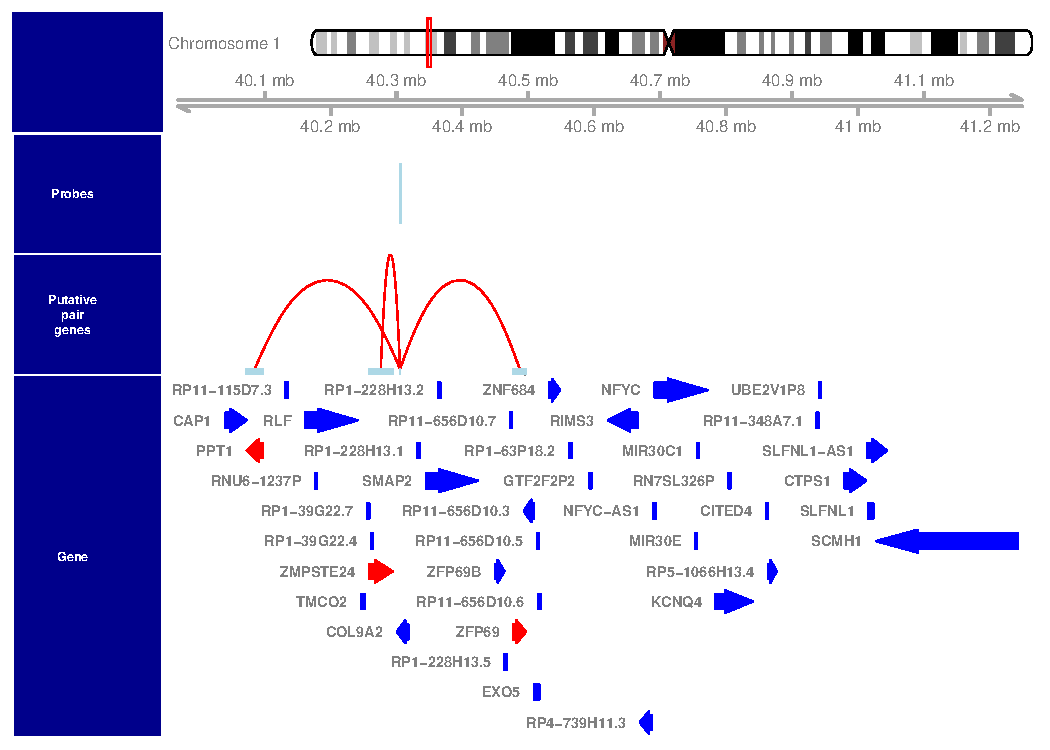
\includegraphics[width=1.0\textwidth]{images/chr1_40000429_41070429_schematic_byCoordinate.pdf}
%\caption{\label{fig:boxplot2} Probe cg00001809 DNA methylation boxplot considering molecular subtypes.}
%\end{figure}

%\begin{minipage}{\linewidth}
\lstinputlisting[language=R,basicstyle=\tiny, frame = none, label = {lst:getpair}, caption = "Identify putative target genes for differentially methylated distal probes"]{codes/getpair.R}
%\end{minipage}

The output of this function is shown in table \ref{tab:get.pair}. Probe and GeneID
columns show the significant pair and the column $P_e$ shows the adjusted p-value.
\begin{table}[h!]
\centering
\small
\csvautobooktabular[respect underscore,
					before reading=\sisetup{round-mode=places,round-precision=2},
                    filter expr={test{\ifnumless{\thecsvinputline}{5}}}]{tables/getPair.hypo.pairs.significant.csv}
\caption [Identification of putative target gene(s) for differentially methylated distal probes]{
Identification of putative target gene(s) for differentially methylated distal probes: First three rows of  getPair.hypo.pairs.significant.csv file.
}
\label{tab:get.pair}
\end{table}

To visualize the relationship between the probe-gene pairs inferred, there are two auxiliary functions in ELMER. The function \textit{schematic.plot}, shown in Listing \ref{lst:plotpair}, which will plot genes and probes in a specified genomic region, highlighting the significant pairs identified by plotting a genomic interactions track and highlight the genes in the pair in red (Figure \ref{fig:parplot}). Also,  using the function \textit{scatter.plot} (Listing \ref{lst:scatterplot}) it is possible to visualize the correlation between gene expression and DNA methylation levels at probe (Figure \ref{fig:scatterplot}).
 Finally, an overall summary of the DNA  methylation levels and gene expression levels  can be visualized using the auxiliary function \textit{heatmapPairs}, as shown in Listing \ref{lst:heatmap}. This function creates a heatmap for all samples  as shown in Figure \ref{fig:heatmap}.

%\begin{minipage}{\linewidth}
\lstinputlisting[language=R,basicstyle=\tiny, frame = none,firstline=5,lastline=13,label = {lst:plotpair},caption = "Schematic plot to visualize gene-probe pairs"]{codes/plotpair.R}
%\end{minipage}

\begin{figure}[ht!]
\centering
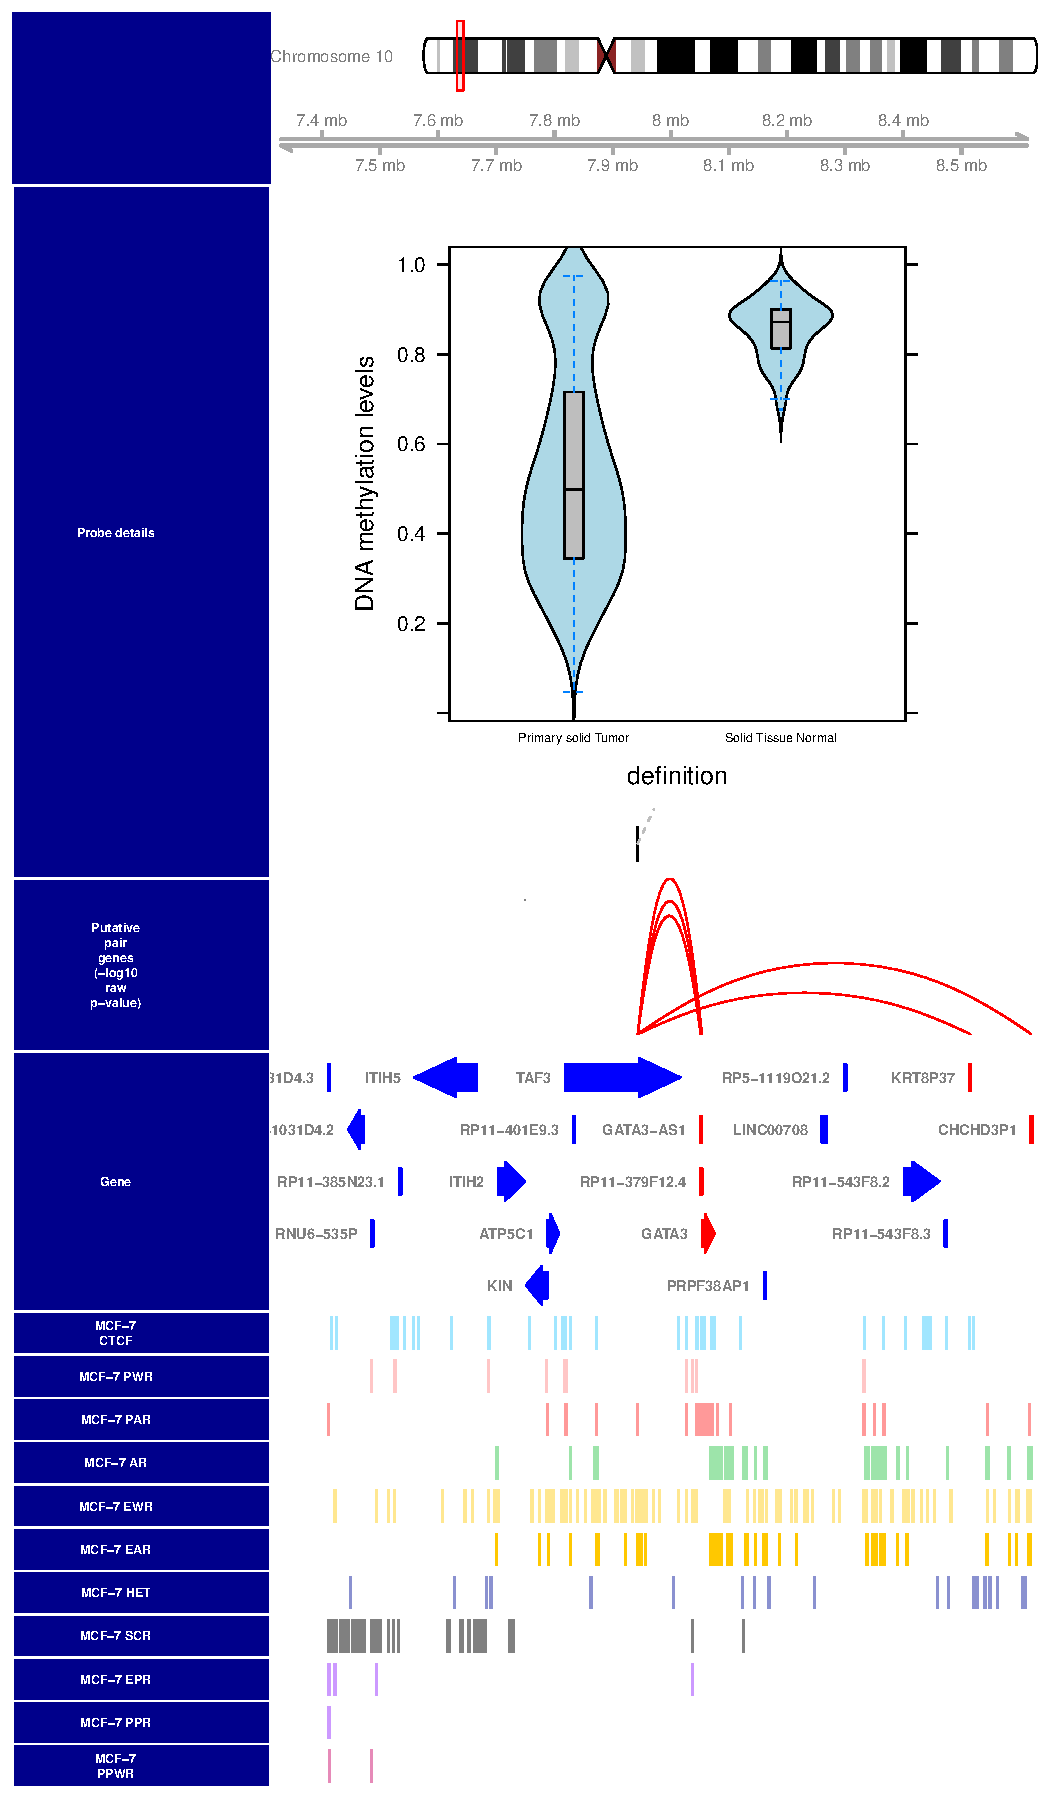
\includegraphics[width=0.7\textwidth]{images/cg04723436_schematic_byProbe.pdf}
\caption[Schematic plot gene-probe pairs]{\label{fig:parplot} Plot probe-gene pairs with annotation track for MCF-7 cell line from \url{StateHub.org}. Significant probes and gene pairs are highlighted in red.}
\end{figure}


% \begin{minipage}{\linewidth}
\lstinputlisting[language=R,basicstyle=\tiny, frame = none,label = {lst:scatterplot},caption = "Scatter plot to visualize correlation between gene expression and DNA methylation levels at probe"]{codes/scatterplot.R}
% \end{minipage}


\begin{figure}[ht!]
\centering
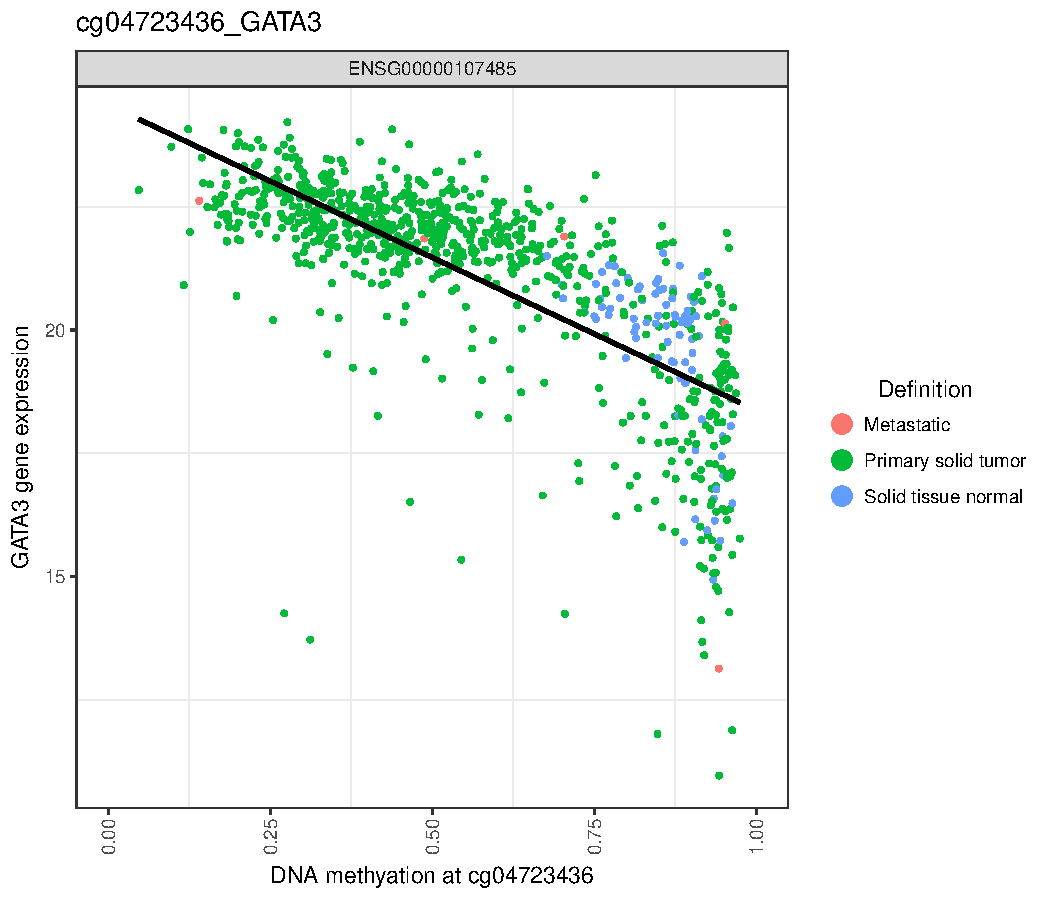
\includegraphics[width=0.7\textwidth]{images/cg04723436_GATA3_bypair.pdf}
\caption{\label{fig:scatterplot} Scatter plot for significant probe (cg04723436) gene (GATA3) pair.}
\end{figure}

\begin{figure}[ht!]
\centering
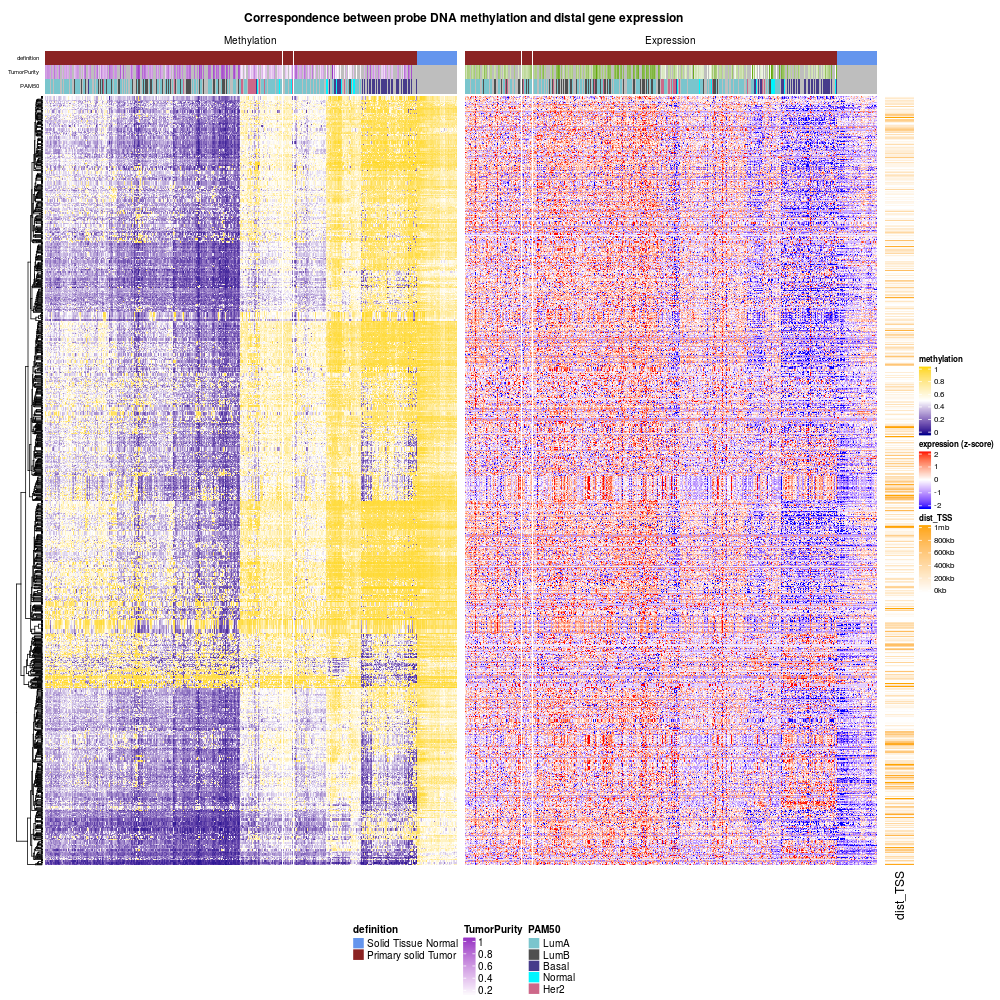
\includegraphics[width=1.0\textwidth]{images/heatmap.png}
\caption{\label{fig:heatmap} Heatmap of paired probes and distal genes. The first heatmap (left one) shows DNA methylation $\beta$ levels ranging from 0 (non-methylated) up to 1 (methylated probes).
The second heatmap (middle one) shows z-scores for gene expression levels (standard deviations from each gene means). The last heatmap (right heatmap) shows the distance between the probe
and gene anti-correlated.}
\end{figure}

\clearpage
\lstinputlisting[language=R,basicstyle=\tiny,frame = none,label = {lst:heatmap},caption = "Heatmap to visualize gene-probe pairs"]{codes/heatmap.R}

\clearpage

\subsection*{Characterization of chromatin state context of significant probe regions using FunciVar}

To understand and compare our set of probes identified in the probe-gene pairs inferred
we used chromatin state of IHEC cell types
from \url{http://statehub.org/}, to calculate the relative enrichment of
different states.
This procedure uses code from the statepaintR \cite{statepaintr} and FunciVar \cite{funcivar} packages.
Figure \ref{fig:funcivar} shows the enrichment for 14 encode cells lines.
The plot shows enrichment for enhancer active region (EAR), weak enhancer (EWR)
and active promoter region (PAR) in MCF-7 cell (human breast adenocarcinoma cell line)
while for other cell lines this enrichment is not visible.

% https://www.ebi.ac.uk/training/online/course/functional-genomics-introduction-embl-ebi-resource/what-functional-genomics-1
%The functional genomics studies investigates a range of processes such as transcription, translation and epigenetic regulation to understand the complex relationship between genotype and phenotype. Among the main issues it tries to elucidate, we can mention  understanding of the regulation of the genes, finding the active gene promoters in a particular cell type and identifying the functional roles of different genes.
%In view of these questions, several international consortia emerged whose objectives could help clarify some of these issues.
%As examples of these consortia we can cite ENCODE (Encyclopedia of DNA Elements) whose objective was to create a comprehensive catalog of candidate functional elements in the genome and REMC (the Roadmap Epigenomics Mapping Centers project), whose objective was to generate reference epigenomic maps for “normal” human cells/tissues.

%These consortia made available a large amount of data such as transcription, transcription factor binding, histone modifications, DNase hypersensitivity, DNA methylation, DNA-DNA interactions, and RNA-protein interactions that have been used to  annotate chromatin state. Listing shows how to use MCF-7 annotation tracks from \url{http://statehub.org/}  to annotate chromatin state of those pairs identified previously.  (see Additional file for the code

%\begin{minipage}{\linewidth}
%\lstinputlisting[language=R,basicstyle=\tiny, frame = none,basicstyle=\ttfamily\scriptsize]{codes/enhancer.R}
%\end{minipage}
%\begin{minipage}{\linewidth}
%\lstinputlisting[language=R,basicstyle=\tiny, frame = none,basicstyle=\ttfamily\scriptsize,label = {lst:funcivar},caption = "Chromatin state annotation for probe regions"]{codes/funcivar.R}
%\end{minipage}

\begin{figure}[ht!]
\centering
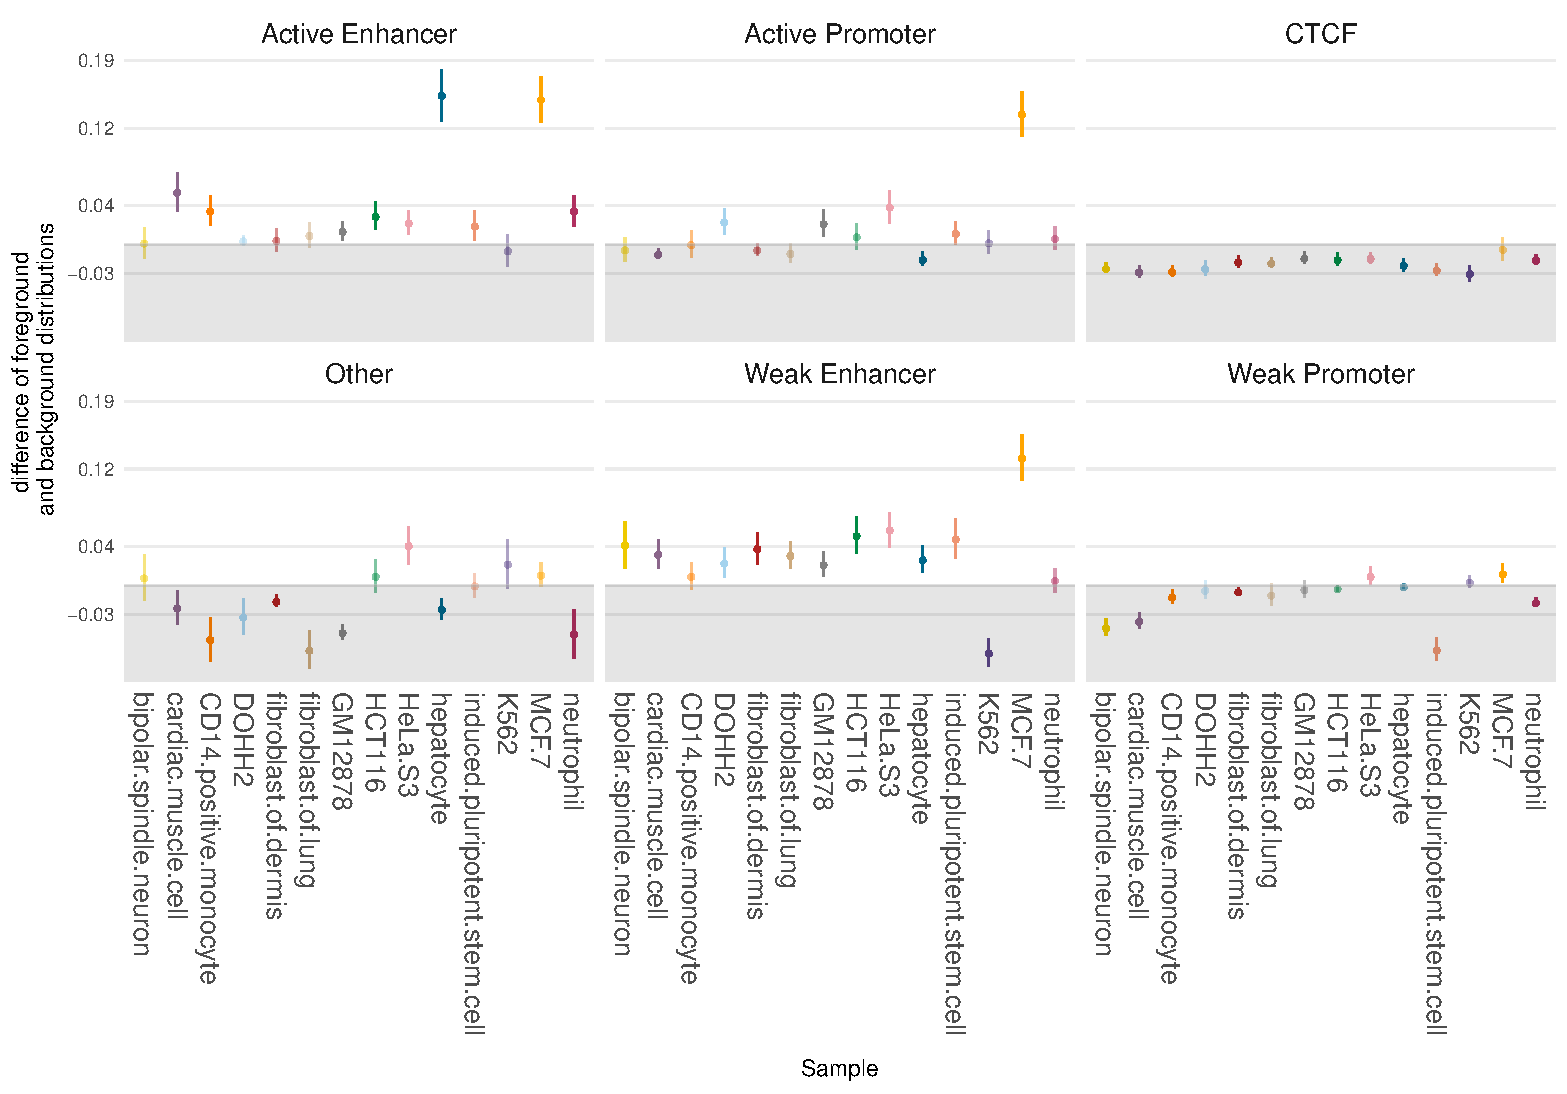
\includegraphics[width=1.0\textwidth]{images/funcivar.pdf}
\caption[ Enrichment of paired probes and chromatin states of encode cells.]{\label{fig:funcivar} Enrichment of paired probes and chromatin states of encode cells.
The plot shows enrichment for enhancer active region, weak enhancer  and active
promoter region for MCF-7 cell. Acronyms - AR: Active region, EAR: active enhancer,
 EWR: Weak Enhancer, EPR: poised enhancer, PAR: active promoter, PWR: Weak Promoter,
 PPR: poised promoter, PPWR: Weak Poised Promoter, CTCF: architectural complex,
 TRS: transcribed, HET: heterochromatin, SCR: Polycomb Repressed Silenced}
\end{figure}


%\cleardoublepage

\subsection*{Identification of enriched motifs within set of probes in significant probe-gene pairs}
The function \textit{get.enriched.motif} is used to identify enriched motif in a set of probes.
The main arguments are described below:
\begin{itemize}
\item \textit{lower.OR}	 The motif with lower boundary of 95\% confidence interval for Odds Ratio $\geq lower.OR$  are the significantly enriched motifs.
\item \textit{min.incidence} Minimum number of probes having the motif signature (default: 10) required for a motif to be enriched.
\end{itemize}

%\begin{minipage}{\linewidth}
\lstinputlisting[language=R,basicstyle=\tiny, frame = none,label = "motif",caption = "Motif enrichment analysis on the selected probes"]{codes/motif.R}
%\end{minipage}

\begin{figure}[ht!]
\centering
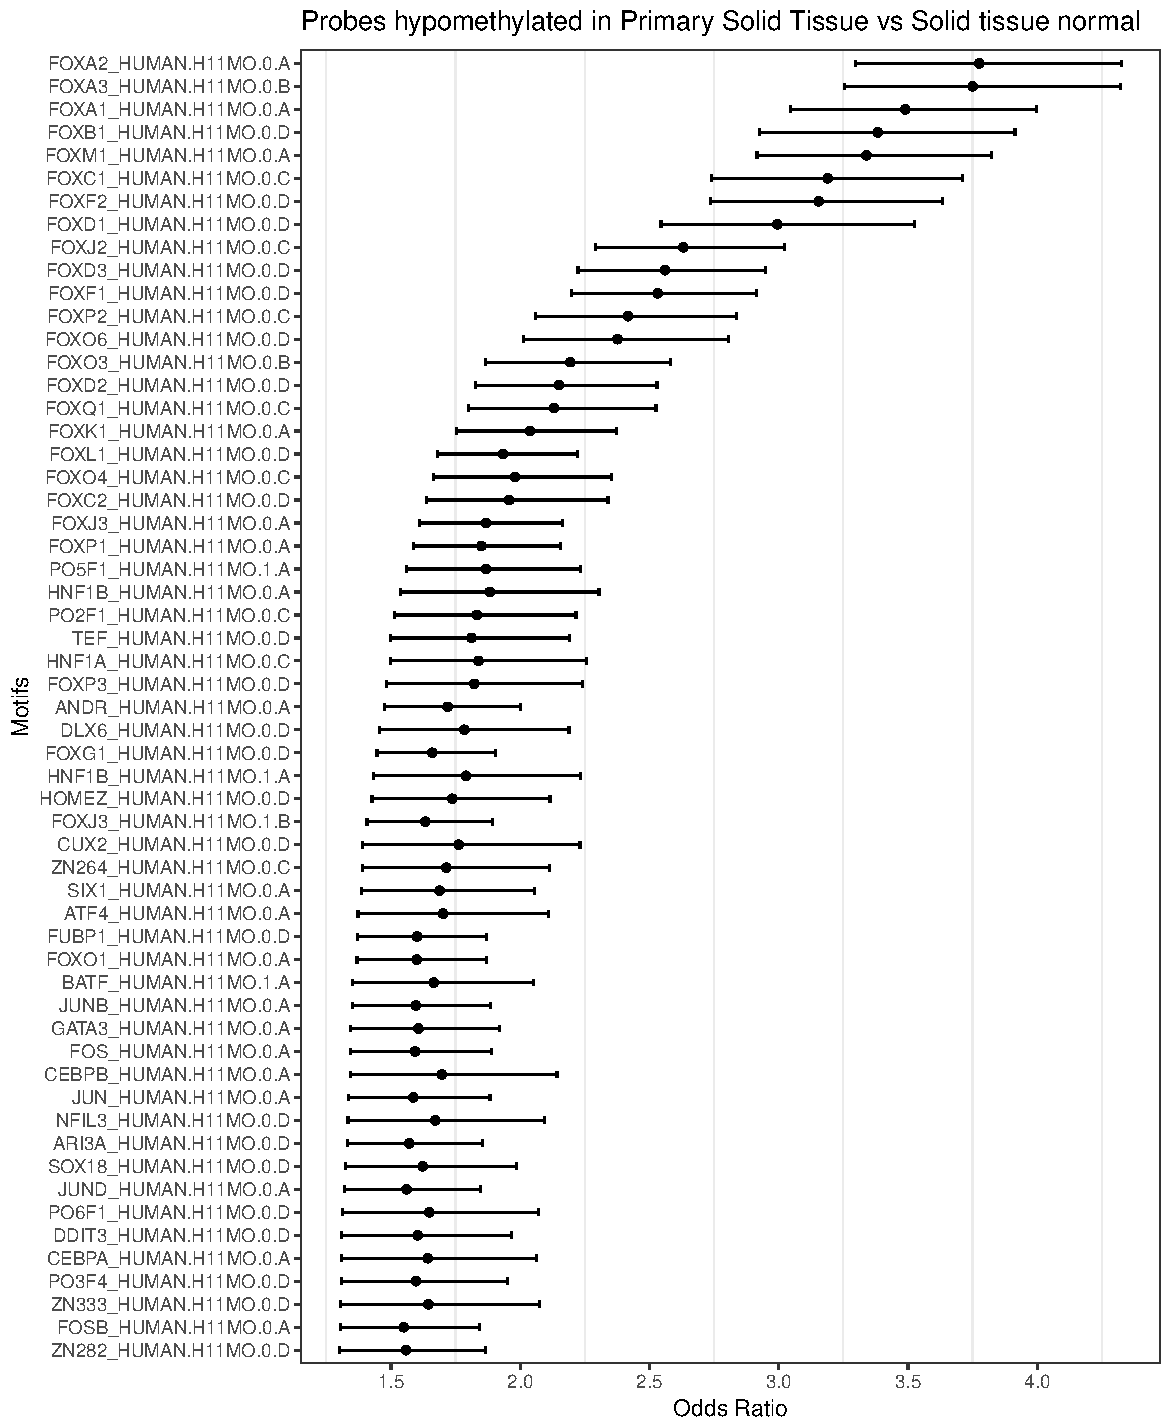
\includegraphics[width=1.0\textwidth]{images/OR_nosummary.pdf}
\caption[Motif enrichment plot]{\label{fig:boxplot2} Motif enrichment plot shows the enrichment levels ($OR\geq2.0$) for the selected motifs. This plot represents a subset of the enriched motifs for $\textit{lower.or}= 1.1$, only selected for representational purposes.}
\end{figure}

\cleardoublepage
\subsection*{Identification of master regulator Transcription Factors (TF) for each enriched motif}
The function \textit{get.TFs} is used to identify regulatory TF whose expression associates with TF binding motif
DNA methylation which.

\lstinputlisting[language=R,basicstyle=\tiny, frame = none,label = "tf",caption = "Identifying regulatory Transcript Factors"]{codes/tf.R}

The result of this function is shown in table \ref{tab:get.tf} and in figure \ref{fig:tfplot}.

\begin{landscape}

\begin{table}[h!]
\centering
\small
\csvautobooktabular[respect underscore,
					before reading=\sisetup{round-mode=places,round-precision=2},
                    filter expr={test{\ifnumless{\thecsvinputline}{20}}}]{tables/getTF.hypo.significant.TFs.with.motif.summary.csv}
\caption[Identification of master regulator Transcription Factors (TF) for each enriched motif] {First twenty rows of  the \textit{getTF.hypo.significant.TFs.with.motif.summary.csv} file created by \textit{get.Tfs} function (suffix "\_HUMAN.H11MO" was removed from motifs names). First column shows the enriched motif, "top\_5percent\_TFs" shows the top 5\% TFs ranked (the same as all TFs to the left of the dashed line in figure \ref{fig:tfplot}), "potential.TFs.family" are the TF from the "top\_5percent"  that belongs to the same family as the TF of the motif, "top.potential.TFs.family" is the highest ranked TF belonging to the same family as the TF of the motif (same as the first TF from "potential.TFs.family" column). The columns "potential.TFs.subfamily" and "top.potential.TFs.subfamily" are the same as "potential.TFs.family" and "top.potential.TFs.family"  but considering the subfamily classification instead. For example, the motif ANDR has two TFs in the top 5\% that belongs to the same TF family (Steroid hormone receptors): ESR1 and AR, but if considering subfamilies only AR in considered.
}
\label{tab:get.tf}
\end{table}
\end{landscape}


\begin{figure}[ht!]
\centering
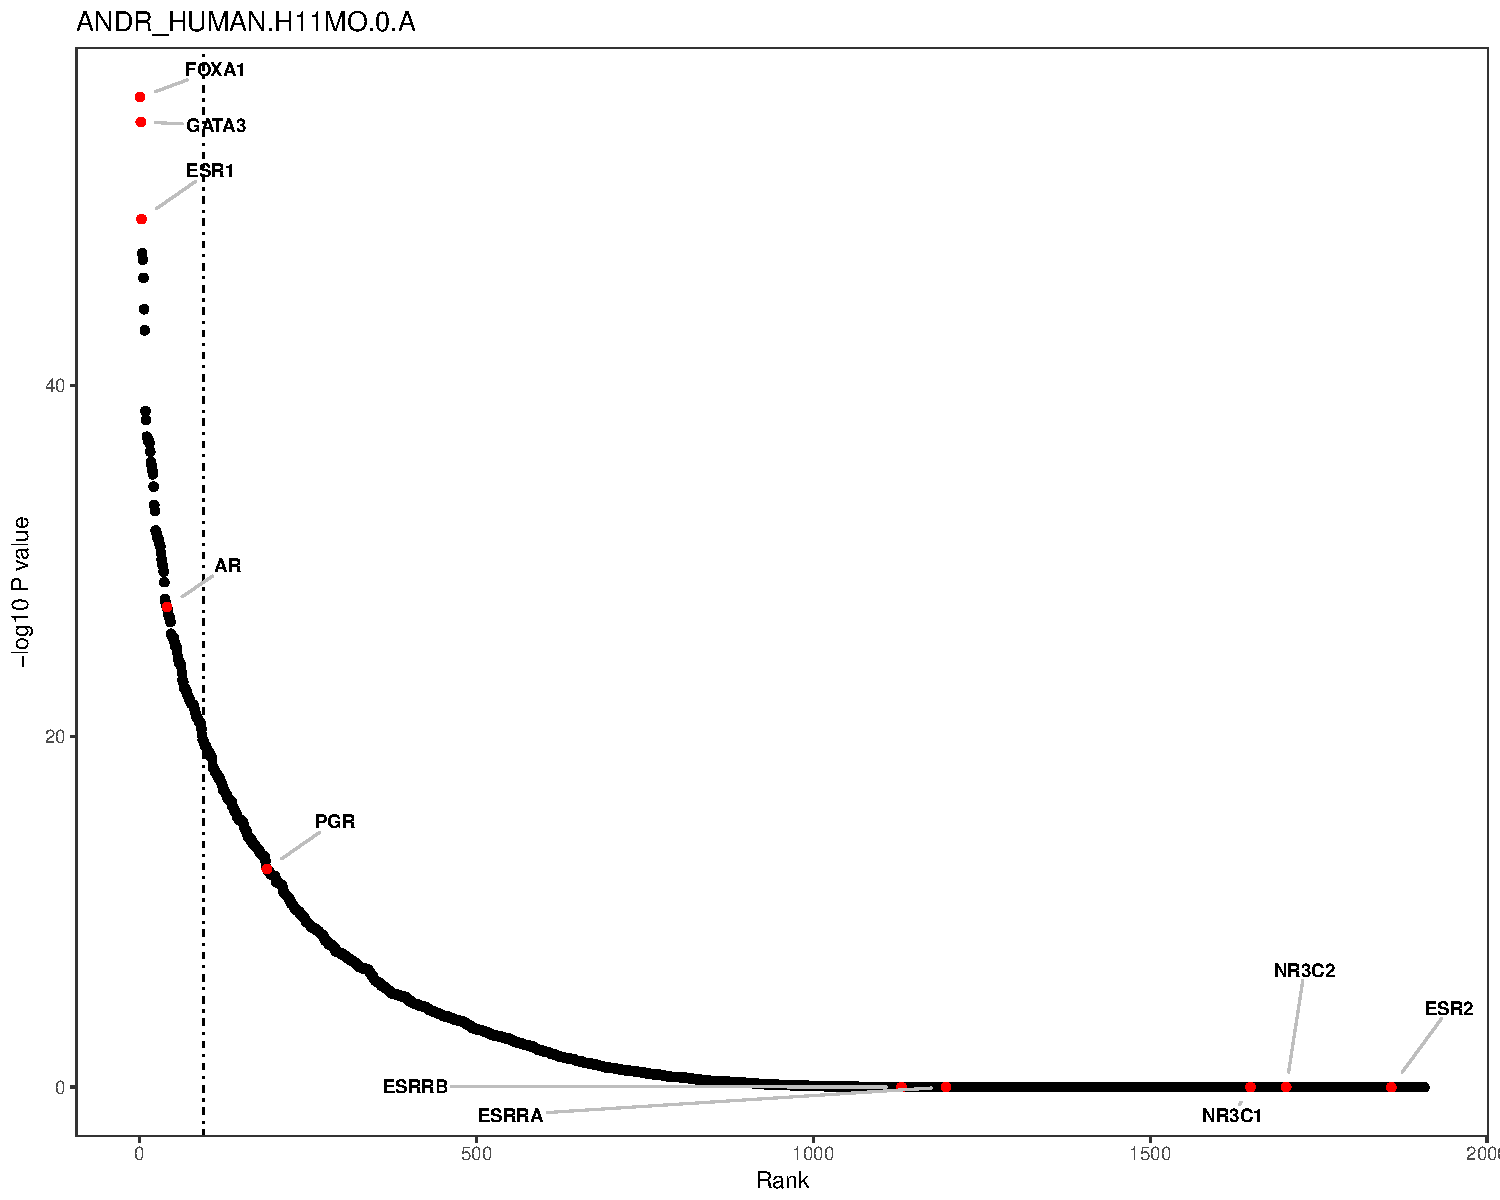
\includegraphics[width=1.0\textwidth]{images/ANDR_HUMAN_H11MO_0_A_TFrankPlot.pdf}
\caption[TF ranking plot: ANDR motif]{\label{fig:tfplot} TF ranking plot shows statistic $-log_{10}(P-value)$ assessing the anti-correlation level
of TFs expression level with average DNA methylation level at sites with a given motif. By default, the top 3 associated TFs and the TF family members (dots in red) that are associated with that specific motif  are labeled in the plot.
But there is also an option to highlight only TF sub-family members (TCClass database classification)}
\end{figure}

\newpage


\subsection*{Comparing inferred results with MCF-7 chIA-PET}

As shown in \citeonline{yao2015inferring}, we compared the putative pairs inferred to the chromatin loops derived from deep-sequenced ChIA-PET data from MCF7 cells \cite{li2012extensive}. First, we identify the number of \textit{ELMER} pairs overlapping the ChIA-PET loops, then we repeat using randomly generated  pairs with properties similar to the \textit{ELMER} pairs. For each true ELMER probe in a probe-gene pair, we randomly select a different probe from the complete set of distal probes. We then choose the nth nearest gene to the random probe, where n is the same as the adjacency of the true ELMER probe (i.e. if the true probe is linked to the second gene upstream, the  random probe will also be linked to its second gene upstream). Thus, the random linkage set has both the same number of probes and the same number of linked genes as the true set. One hundred such random datasets were generated to arrive at a 95\% CI ($\pm 1.96* SD$).
The result is shown in Figure \ref{fig:chiapet}. Of the 2124 putative pairs identified in breast cancer tumors, 316 (approximately 14.9\%) were also identified as loops in the MCF7 ChIA-PET data. This was a three-fold enrichment over randomized probe-gene pairs (see Additional file for the code).


%\begin{minipage}{\linewidth}
%\lstinputlisting[language=R]{codes/mcf7-validation.R}
%\end{minipage}

\begin{figure}[ht!]
\centering
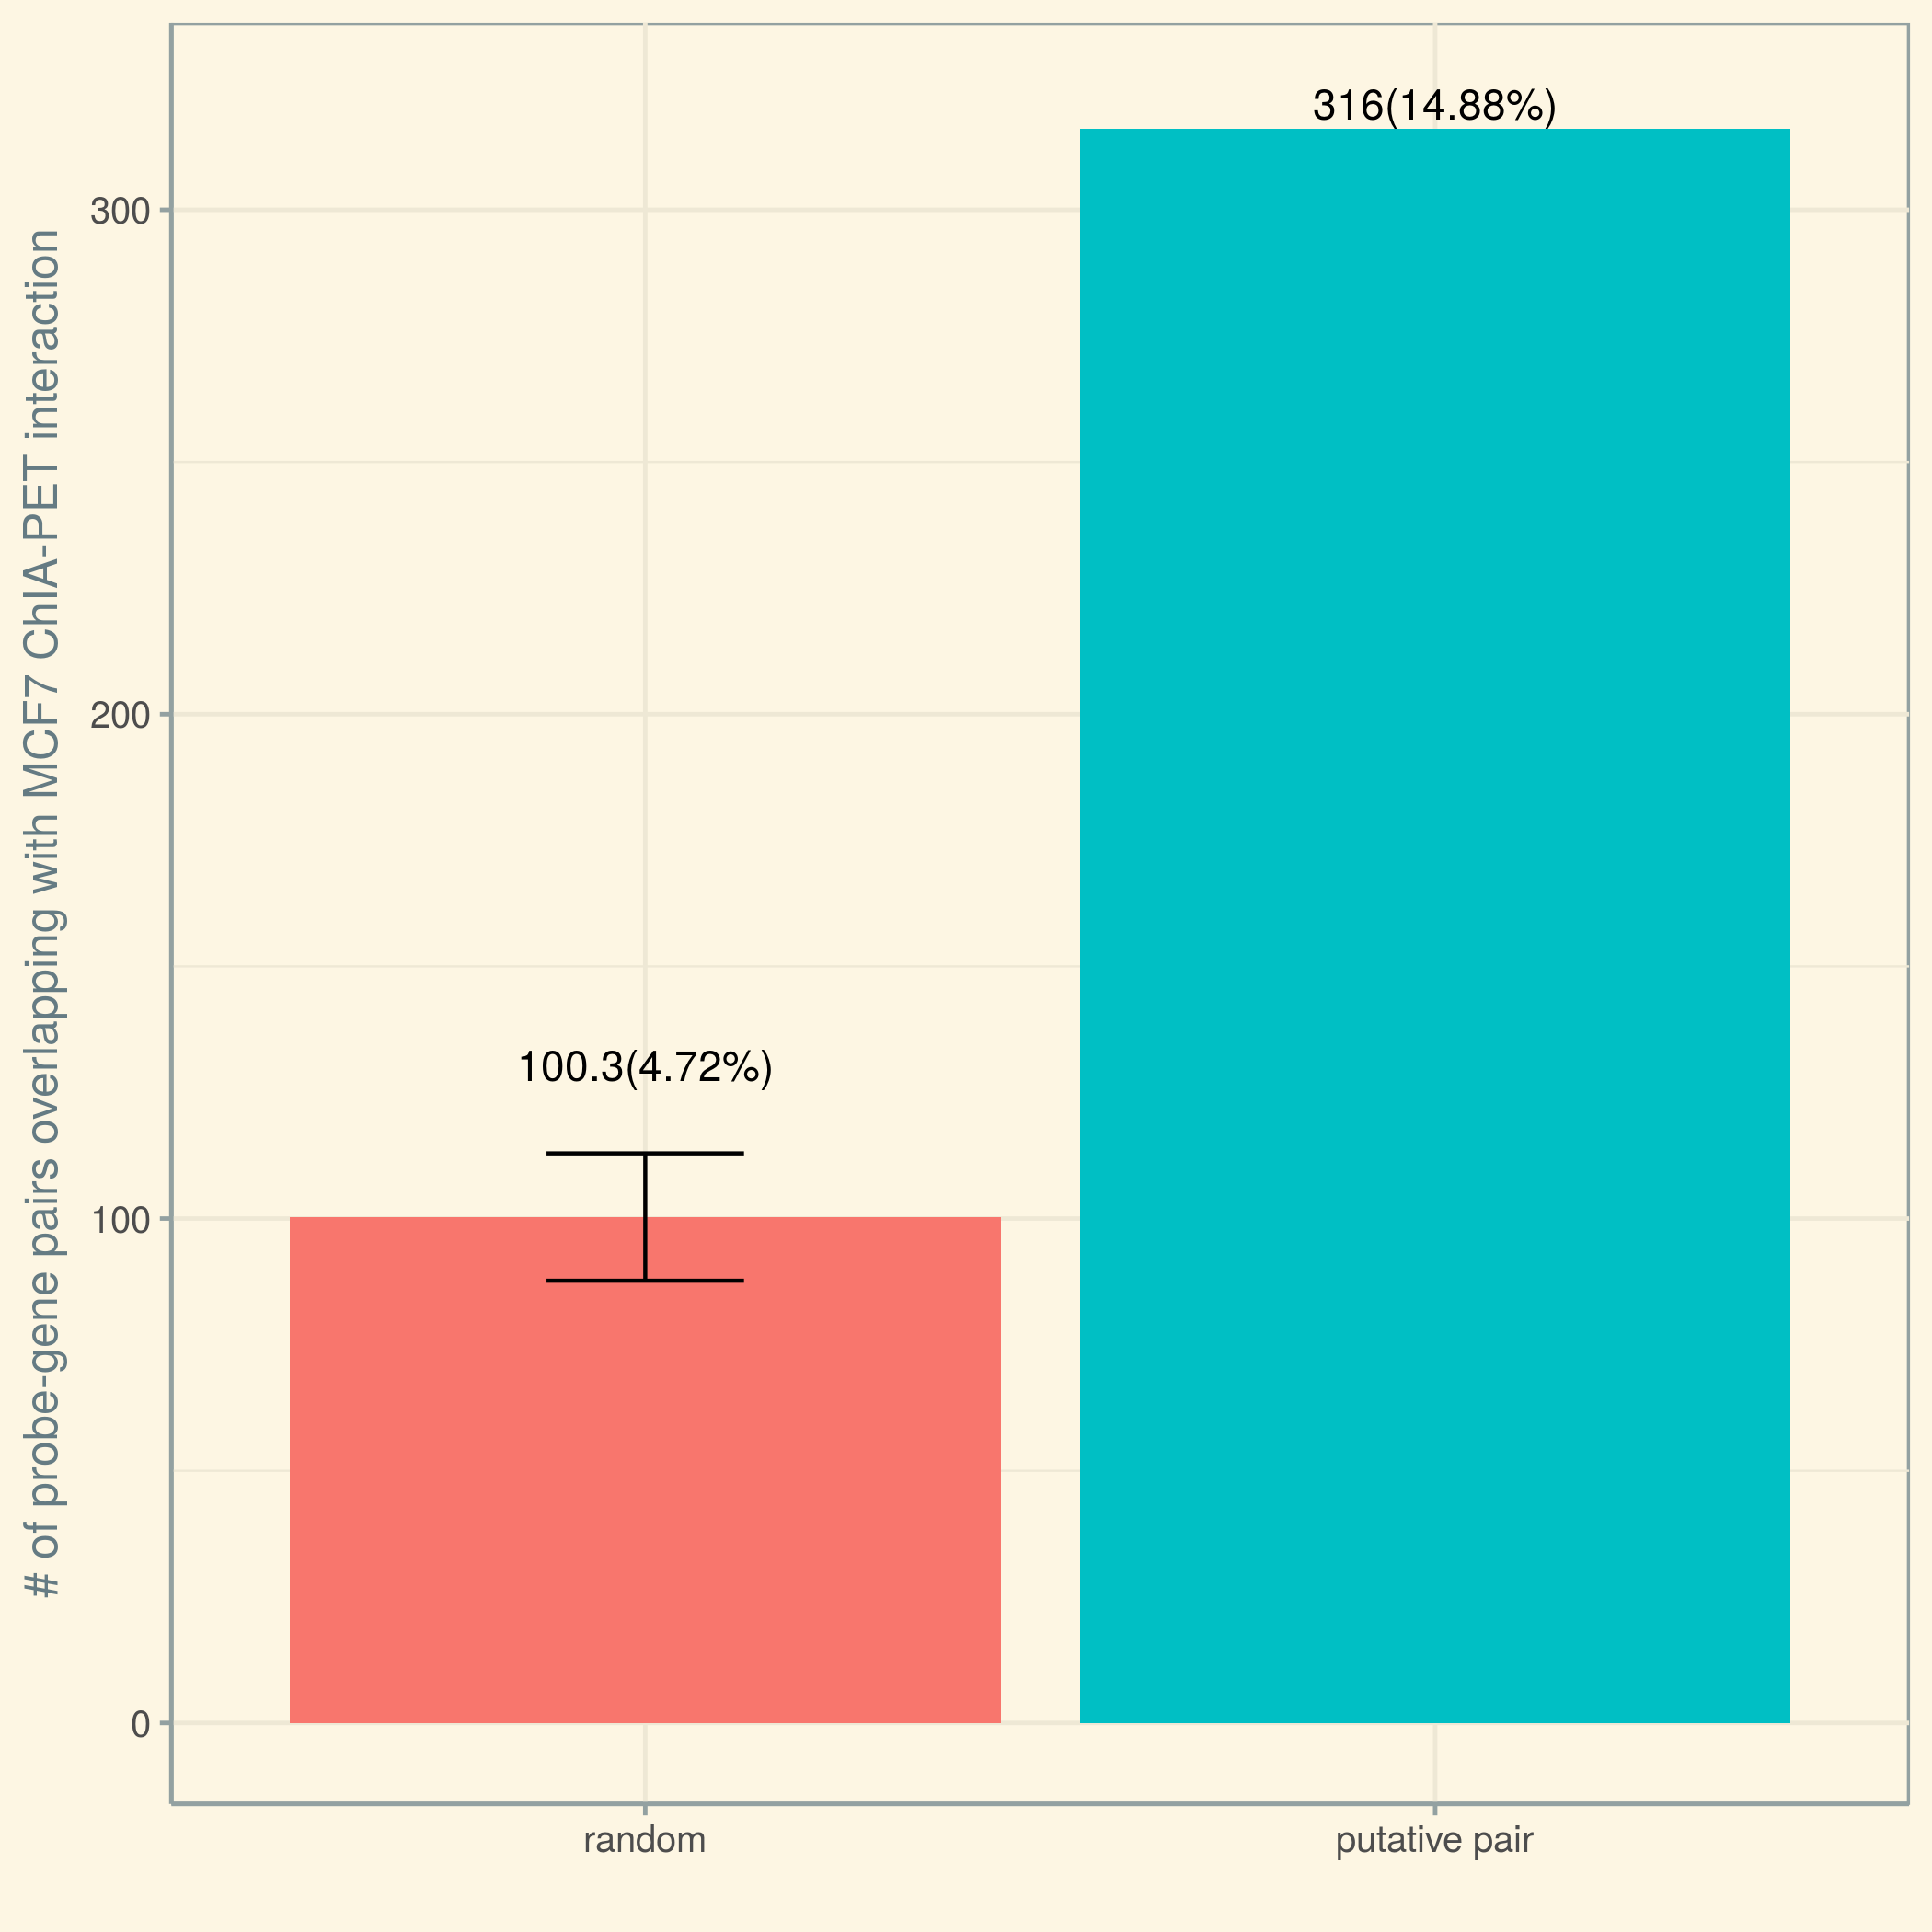
\includegraphics[width=0.6\textwidth]{images/validation.png}
\caption[MCF7 ChIA-PET validation]{\label{fig:chiapet} The graph shows the comparison of the number of probe-gene pairs identified within MCF7 ChIA-PET data using the putative pairs from BRCA vs. random pairs}
\end{figure}


\clearpage
\subsection{Use Case 2: BRCA molecular subtypes analysis (supervised approach)}

Several studies identified distinct molecular Breast cancer classes and
divided them as the luminal-like (Luminal A and Luminal B) subclasses,
which are Estrogen receptor-positive (ER-positive), and the basal-like,
ErbB2-positive and normal-like subclasses, which are the ER-negative
groups \cite{perou2000molecular,yersal2014biological,sorlie2001gene}.
To performed \textit{ELMER} analysis comparing known molecular subtypes
(Her2, Luminal A, Luminal B and Basal-like) a TCGA BRCA dataset classification
retrieved from \citeonline{ciriello2015comprehensive}.


The main arguments changed were the percentage of samples used to identify the
differentially methylated probes in function \textit{get.diff.meth} which was
set to 100\% (use all samples from each group) and the mode in function \textit{get.pair}
and in function \textit{get.TFs} which was set to "supervised". In this mode instead
of defining the U (unmethylated) group as the samples with lowest quintile of DNA
methylation levels and the M (methylated) group as the highest quintile, the $U$ and $M$ group
 will be defined as all samples of one known molecular subtype.
 For example, if the first step identified probes hypomethylated in Luminal A group compared to Basa-like group,
in the next steps the U group will be the Luminal A samples and the M group will be the Basal-like samples.
The results and code of this supervised analysis can be found in the supplemental files,
a venn diagram with the candidate TF actives in each molecular subtype are shown in Figure \ref{fig:venn}.

From the  Luminal A group vs Basal-like group analysis, it can be highlighted that the pairs of
high expressed genes and hypomethylated probes in the Basal groups are enriched for the SOX10 TF signature.
For this signature, the regulatory TF candidate identified is the SOX11 (Sry-related HMG box-11) TF; this
correlation between basal-like and SOX11 was recently described by \citeonline{shepherd2016sox11}.
Also, the TF analysis  reported the forkhead box C1 (FOXC1) transcription factor as the TF with the
highest anti-correlation between TF expression and DNA methylation levels. Even though,
this TF is not in the family of any enriched motifs this correlation between the FOXC1 TF and Basal-like
breast cancers (BLBCs) was reported by \citeonline{zuo2016role} and \citeonline{chung2017identification}.

On the other hand, when analyzing in the other direction in terms of methylation level, for  those pairs of high expressed genes and hypomethylated probes in the Luminal A group, the TF analysis identified GATA3, FOXA1, RARA, MYB as candidate regulatory TF. GATA3 and FOXA1 are known characterize this  molecular subtype  as described by \citeonline{yersal2014biological} while RARA was associated with the Luminal phenotype by \citeonline{centritto2015cellular}, MYB
is shown to be required for the proliferation of ER-positive breast cancer cells \cite{mitra2016cdk9}.

\begin{figure}[ht!]
\centering
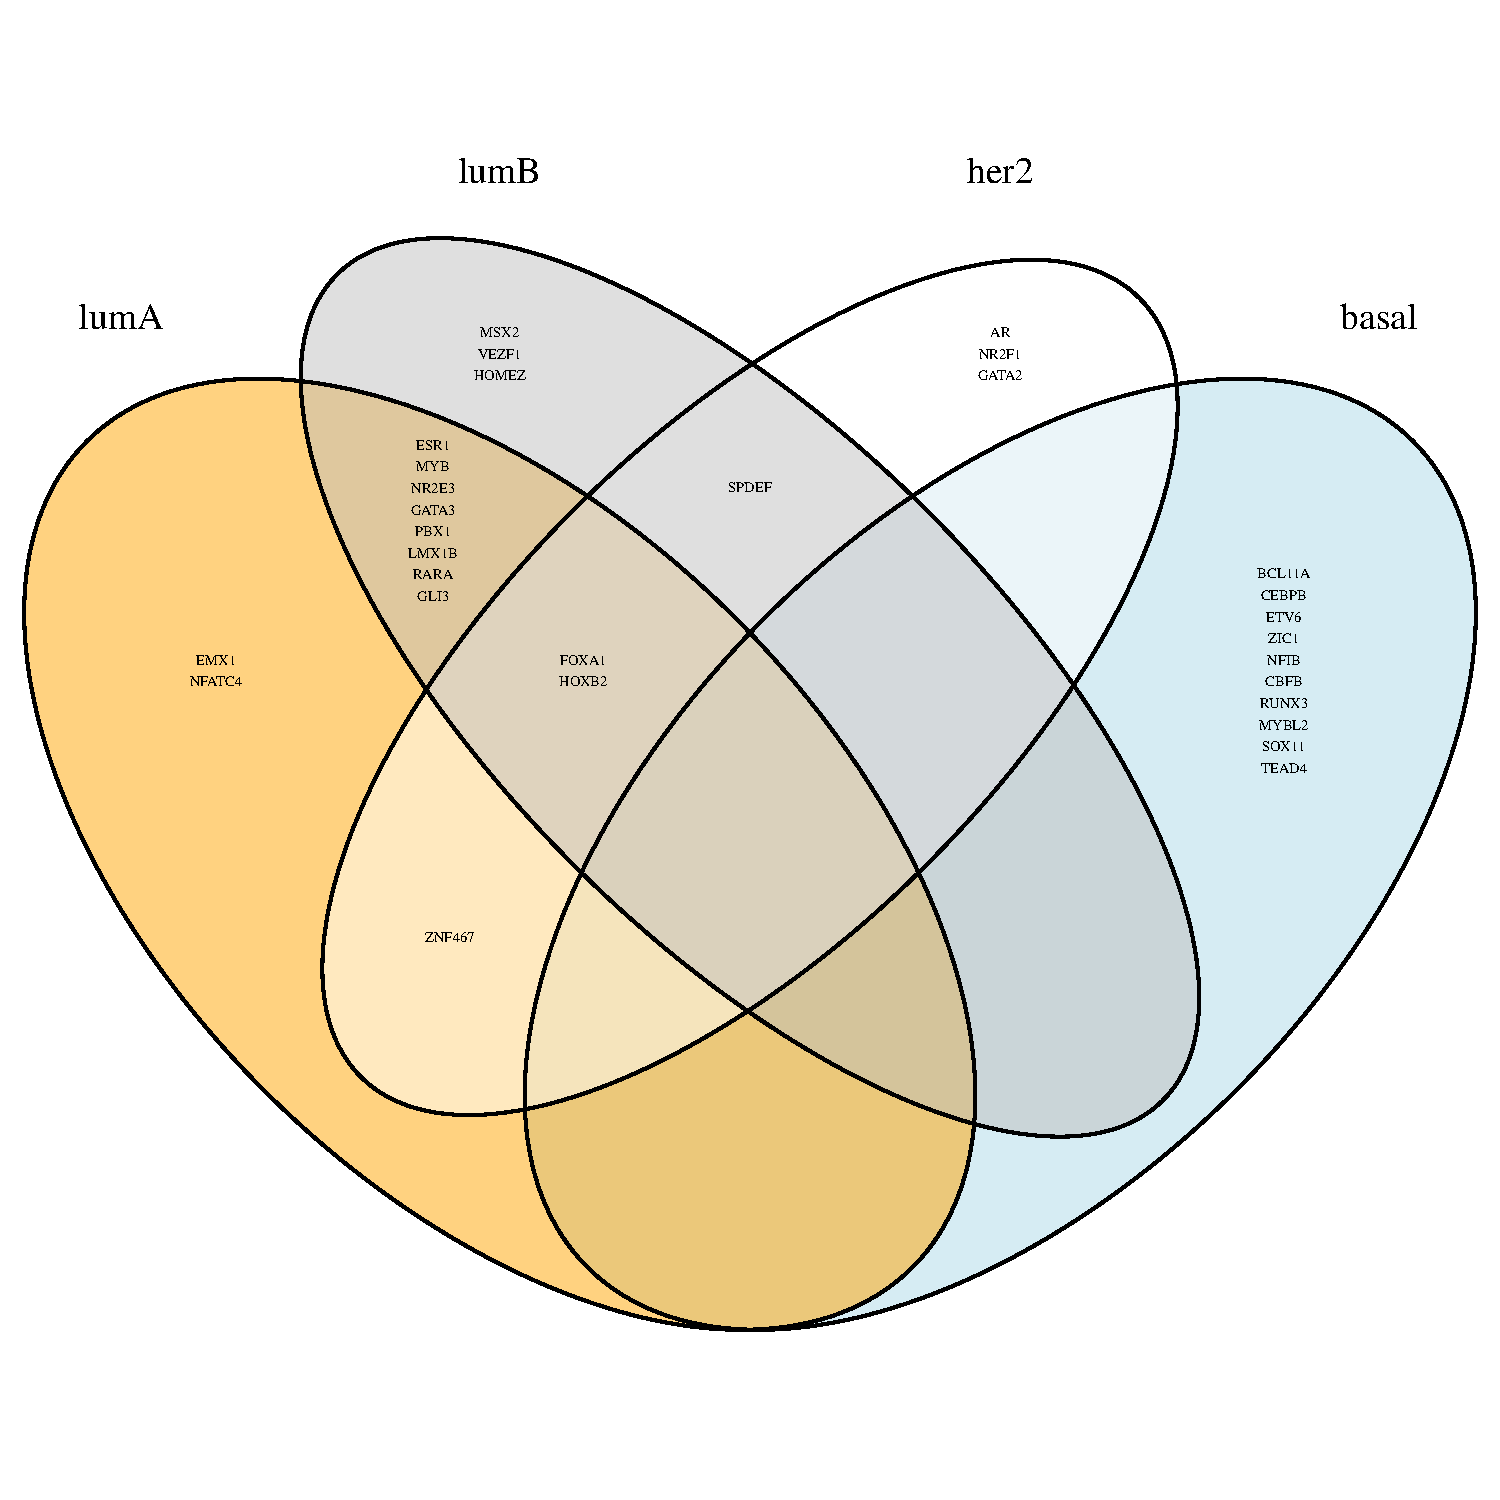
\includegraphics[width=1.0\textwidth]{images/BRCA_ven.pdf}
\caption{\label{fig:venn} Venn diagram of candidate regulatory TFs for each molecular subtype found in at least one of the pairwise comparisons.}
\end{figure}

\section*{Data availability} % Optional - only if novel data or analyses are included
The TCGA data was downloaded from the NCI Genomic Data Commons (GDC) data portal \cite{grossman2016toward}
using TCGAbiolinks R/Bioconductor package \cite{colaprico2015tcgabiolinks,10.12688/f1000research.8923.2}.
Gene annotations were retrieved from ENSEMBL \cite{yates2015ensembl} database via biomaRt R/Bioconductor
package \cite{durinck2005biomart,durinck2009mapping}.
DNA methylation microarrays metadata were retrieved from \url{http://zwdzwd.github.io/InfiniumAnnotation} \cite{doi:10.1093/nar/gkw967}.
Transcription factor (TF) binding models can be downloaded at HOCOMOCO database (\url{http://hocomoco.autosome.ru/}) \cite{kulakovskiy2016hocomoco}.
The list of human TF can be accessed at \url{http://www.uniprot.org/}  \cite{apweiler2004uniprot}.
The classification of human transcription factors (TFs) can be viewed at \url{http://tfclass.bioinf.med.uni-goettingen.de/tfclass}  \cite{wingender2013tfclass}.

\section*{Software availability}

ELMER	source code  is available at \burl{https://github.com/tiagochst/ELMER}
and the auxiliary data files are available \burl{https://github.com/tiagochst/ELMER.data}.
\textit{ELMER} is available under the GNU General Public License version 3 (GNU GPL3).
